\documentclass{article}
\usepackage[a4paper, left=2cm, right=2cm, top=1.5cm, bottom=1.5cm]{geometry}
\usepackage[heading=true, zihao=-4, UTF8]{ctex}
\usepackage{setspace}
\usepackage{graphicx}     %插入图片的宏包
\usepackage{float}        %设置图片浮动位置的宏包
\usepackage{abstract}     %设置摘要样式
\usepackage{caption}      %标签
\usepackage{booktabs}
\usepackage{multirow} % 用于合并单元格(可选)
\usepackage{fontspec}   %设置英文字体
\usepackage{titletoc}     %设置目录样式
\usepackage{amsmath}
\usepackage[super, square]{natbib}

\setmainfont{Times New Roman} %设置英文字体

\let\kaishu\relax
\newCJKfontfamily\kaishu{KaiTi}[AutoFakeBold]
\let\songti\relax
\newCJKfontfamily\songti{SimSun}[AutoFakeBold]

\ctexset{
  section = {
    format += \zihao{3} \heiti \mdseries,
    aftername = \hspace{0.5em}
  },
  subsection = {
    format += \zihao{-3} \heiti \mdseries,
    aftername = \hspace{0.5em}
  } ,
  subsubsection = {
    format += \zihao{4} \heiti \mdseries,
    aftername = \hspace{0.5em}
  }
}

\renewcommand{\contentsname}{\zihao{3}\heiti\mdseries 目\ \ \ 录}
\titlecontents{section}[0pt]{\vspace{0.25\baselineskip} \mdseries \zihao{-4}}{\contentslabel{1em}}{}{\titlerule*[0.25pc]{.} \contentspage}
\titlecontents{subsection}[2.6em]{\vspace{0.25\baselineskip} \mdseries \zihao{-4}}{\contentslabel{1.6em}}{}{\titlerule*[0.25pc]{.} \contentspage}
\titlecontents{subsubsection}[4.3em]{\vspace{0.25\baselineskip} \mdseries \zihao{-4}}{\contentslabel{2.3em}}{}{\titlerule*[0.25pc]{.} \contentspage}

\renewcommand {\thetable} {\thesection{}-\arabic{table}}    %设置表格编号与章节对应
\renewcommand {\thefigure} {\thesection{}-\arabic{figure}}  %设置图片编号与章节对应
\numberwithin {equation}{section}

\captionsetup {
  font={
    small,
    stretch=1.25
  },
  labelsep=space
}

\begin{document}
\zihao{-4}

\pagestyle{empty} %自定义封面
\begin{center}
  {\zihao{-4} \hspace{1em} \\ \vspace{1em}}
  {\zihao{0} \songti 珠海科技学院 \\ \vspace{1em}}
  {\zihao{0} \songti \textbf{毕\ 业\ 设 \ 计} \\ \vspace{1em}}
  {\zihao{-1} \kaishu \textbf{基于FPGA的JPEG图像编码系统设计} \\ \vspace{4em}}
  \zihao{-2}
  \kaishu
  \makebox[10em][s]{学院:}\ {\makebox[10em][l]{电子信息工程学院}}\\
  \makebox[10em][s]{专业名称:}\ {\makebox[10em][l]{微电子科学与工程}}\\
  \makebox[10em][s]{学生姓名:}\ {\makebox[10em][l]{黄智为}}\\
  \makebox[10em][s]{学号:}\ {\makebox[10em][l]{03210828}}\\
  \makebox[10em][s]{指导老师姓名、职称:}\ {\makebox[10em][l]{孙永坚\ 讲师}}\\
  \vspace{1em}
  {\zihao{4} \heiti 完成日期:\today}
\end{center}
\clearpage


\newpage
\pagestyle{plain} 
\setcounter{page}{1}
\pagenumbering{Roman}

\renewcommand{\abstractnamefont}
  {\centering\zihao{-4}\normalfont\sffamily}
  \renewcommand{\abstractname}{\zihao{3} \heiti 摘\ \ \ 要}
  \addcontentsline{toc}{section}{摘要}
\begin{abstract}
  \zihao{-4}
  随着近几十年来多媒体技术、图像扫描技术、移动终端、通信技术的不断发展,数
  字图像和视频数据的广泛使用,图像数据的数量呈指数机增加。于此对图像数据的
  存储以及传输的需求日益严峻。一味地添加设备的存储容量和信道的带宽是不现实
  的,对此使用图像压缩技术来减少图像数据的数据量。而作为静态图像压缩国际标
  准格式的JPEG(Joint Photographic Experts Group),因具有压缩率高、失真率
  小等特点。在国际上取得广泛的应用。

  目前大多数的JPEG格式图像数据编解码系统都是基于软件编程从而运行在通用计算
  机上。这种方式存在计算效率低、实时性低、运行功耗高等诸多缺点。于此同时具
  有对硬件可编程、运行功耗低的FPGA(Field Programmable Gate Array)芯片的
  规模不断增加,在FPGA芯片内实现复杂的数字信号处理系统已成为现实。因此本设
  计将JPEG压缩技术和FPGA相结合提升系统的性能,并从实际工程出发,设计出一套
  JPEG编码系统。完成JPEG编码在FPGA上的实现。

  本论文的结构首先阐述了JPEG格式的编码FPGA实现的研究背景与意义国内外研究
  现状,并以此使用了一种的基于脉动阵列实现DCT算法的流水线结构。接着描
  述了JPEG格式编码和解码算法的实现步骤。然后采用SOC的设计思想,给出整个硬
  件系统的内部结构、层次划分,对每个运算步骤进行了详细的描述。最后完成整体
  的验证。 

  本设计基于Xilinx的Zynq系列的FPGA的硬件平台,对上位机输出的rgb格式的图像进
  行采集和压缩,再通过使用低速串行通信协议传输压缩数据。在EDA 工具vivado2019.1
  中完成综合仿真、布局布线以及码流生成。 \vspace{1em} \\
  \noindent\textbf{\songti 关键词:} FPGA;图像压缩;JPEG
\end{abstract}

\newpage

\renewcommand{\abstractnamefont}
  {\centering\large\normalfont\sffamily}
  \renewcommand{\abstractname}{ABSTRACT}
  \addcontentsline{toc}{section}{ABSTRACT}
\begin{abstract}
  With the continuous advancement of multimedia technology, image scanning technology, 
  mobile terminals, and communication technology in recent decades, the widespread use
  of digital images and video data has led to an exponential increase in the volume of image 
  data. Consequently, the demand for storage and transmission of image data has become 
  increasingly critical. Simply increasing the storage capacity of devices and the bandwidth 
  of communication channels is impractical. Therefore, image compression technology is 
  employed to reduce the volume of image data. JPEG (Joint Photographic Experts Group), 
  as the international standard format for static image compression, is widely adopted globally due to its high compression ratio and low distortion rate.

  Currently, most JPEG image data encoding and decoding systems are based on software programming and run on general-purpose computers. This approach has several drawbacks, including low computational efficiency, poor real-time performance, and high power consumption. At the same time, the scale of FPGA (Field Programmable Gate Array) chips, which are hardware-programmable and have low power consumption, has been continuously increasing. Implementing complex digital signal processing systems within FPGA chips has become a reality. Therefore, this design combines JPEG compression technology with FPGA to enhance system performance and, based on practical engineering considerations, designs a JPEG encoding and decoding system. This system achieves the implementation of JPEG encoding and decoding on an FPGA.

  The structure of this thesis first elaborates on the research background and significance of implementing JPEG format encoding and decoding on FPGA, as well as the current research status both domestically and internationally. Based on this, a novel pipelined structure for implementing the DCT algorithm using a systolic array is proposed. Subsequently, the implementation steps of the JPEG format encoding and decoding algorithms are described. Then, adopting the System-on-Chip (SOC) design philosophy, the internal structure and hierarchical division of the entire hardware system are presented, with detailed descriptions of each computational step. Finally, the overall verification is completed.

  This design is based on the Xilinx Zynq series FPGA hardware platform, which captures and compresses image data from the CMOS image sensor OV5640. The compressed data is then transmitted using a low-speed serial communication protocol. The synthesis, simulation, layout, routing, and bitstream generation are completed in the EDA tool Vivado 2019.1.

    \noindent\textbf{keywords:} FPGA; JPEG; image compression 
\end{abstract}

\newpage
\tableofcontents

\newpage
\setcounter{page}{1}
\pagenumbering{arabic}

\begin{spacing}{1.25} %设置行距离
\section{绪\ \ 论}
  \subsection{研究背景及研究意义}
    \vspace{1em}
    图像数据作为信息的重要载体,在如今这个信息化的社会扮演着不可欠缺的角色
    相对与文本,图像具有强大的表达能力,通过像素、色彩及形状结构等元素传递
    出大量的信息。而数字成像设备捕获和处理的图像对人们生活和生产活动在各个
    方面产生直接影响。\cite{数字图像处理MATLAB版本科教学版}随着高清图像和视
    频的普及,图像数据的数量呈指数级增长。对高存储空间传输带宽的需求日益严
    峻。以分辨率为1920×1080的24位像素深度的60刷新率的视频数据为例,如果使用
    原像素数据进行存储。1GB的存储空间仅能够存储6秒左右的视频片段。因此一味地
    添加设备的存储容量和信道的带宽是不现实的,由此图像压缩技术孕育而生。该
    技术通过图像数据存在大量的冗余的特性,对图像数据进行压缩编码。

    目前图像压缩格式应用最广的是JPGE压缩格式。它运用图像数据在空间上的连续
    性,空间上存在一定程度的冗余性;以及人眼对图像的辨别度有限,即在视觉上
    存在一定程度的冗余性;最后有些图像中包含了一些先验知识有关的信息,即知
    识冗余性;通过这些特性\cite{1022468688.nh}来减少图像的数据量。目前JPEG
    图像大多数使用软件进行编解码。但对于医疗器械、自动驾驶、视频监控等对视
    频画面逐帧处理要求高的场景,这种方式有着效率低、运行功耗高等诸多缺点。

    在硬件实现上,业内普遍用图像专用集成电路(Application Specific Intergrated
    Circuit ASIC),但是ASIC缺乏一定的灵活性,不能轻松实现一些差异化的图像
    处理功能。而基于FPGA平台的图像压缩系统是当前研究开发的热点。
    
    本设计采用FPGA高并行计算能力和低功耗的特性设计出一套高效运行的JPGE格式
    编码系统。该系统能保证图像数据高实时传输地同时保持较低的功耗,适合运
    它运用在嵌入式系统或边缘计算设备。通过对算法进行硬件级优化,FPGA能够对
    JPGE压缩的各个环节进行流水线和并行处理。相对于传统的软件开发方式极大地
    提升了系统的吞吐量和响应速度,同时保持较低的运行功耗。此外这种编码系
    统作为软核结合FPGA使用使用具有较强的可扩展性,可与大多数视频图像处理系
    统相结合,助力更多地创新应用开发。
  \subsection{国内外研究现状}
    \vspace{1em}
    随着近几十年来信息技术地不断发展,图像和视频数据被广泛运用。因此如何降
    低数据的存储大小和传输系统的负担一直是研究的问题。现如今图像数据压缩编
    码主要分为两种,一种是针对静止图像在空间在空间的纬度上进行压缩编码的压
    缩方式,如JPEG、JPEG-2000、JPEG-LS。另一种是针对多个数据帧在时间纬度上
    进行压缩的方式如H.264、H.256\cite{sze2014high}等。其中JPEG(Joint Phot
    ographic Exprts Group,联合专家组)标准有ISO在1991年提出\cite{pennebaker1992jpeg},
    之后有相继提出了JPEG-L、JPEG-Motion、JPEG2000三个图像标准,JPEG-LS是一
    种接近无损压缩的压缩格式,其工作简单高效,但是输出的编码率随原图像的改
    变存在较大的波动。PEG-MONTION是基于JPEG发展起来的,可用于动态图像的压缩,
    但是压缩率比较低。JPEG2000是用小波变换代替JPEG的离散余弦变换(DCT),在
    低比特率下,有更良好的图像压缩性能,但是算法的复杂度高,因此在一下追求
    低负责度的实时应用中,JPEG2000无法替代JPEG,在大多数的场合之下,使用JPEG
    就能满足需要了。

    国外在jpeg硬件编解码方面的研究成果有:在使用ASIC上,美国AD公司推出的高性能
    图像编解码芯片AD212是。支持JPEG和JPEG2000图像格式的编解码,在JPEG编解码方面
    器核心DCT变换基于优化的8×8定点运算架构,能够处理完成正向和反向DCT计算,同时
    通过可编程量化表支持动态调整,使用者可以更具使用需求平衡图像质量和带宽占用
    。在性能方面ADV212的JPEG编码处理速率可达60MSamples/s,能满足1080p分辨率下30fps
    实时处理的需求。对于JPEN格式编解码FPGA实现的研究现状有:里斯本高级工程学院
    的学者\cite{ref10}利用FPGA独有的硬件结构可编程的特点,使用了FPGA动态局部可重
    构技术,根据编码的流程对FPGA硬件逻辑资源进行分时复用,实现硬件资源利用最大化。
    采用该方案相对使用传统的静态解决方案在资源占用上节省了60\%,但代价是是运行速度
    上慢了9倍。Shan等人\cite{ref11}通过行列分解的方式实现2D-DCT(二维离散余弦变换)
    ,并在设计中引入乒乓缓存器。在运行在100MHZ的时钟信号下,针对1920*1080的图像,
    最快解码率可达到30fps的视频刷新率。Teja\cite{teja2015verilog}等人针对2D-IDCT
    (二维离散余弦逆变换)设计了一种全流水的硬件结构,同时不使用乘法器,降低了
    2D-IDCT模块的资源利用。在JPEG解码上的研究主要围绕Huffman解码展开,巴尔伊兰
    大学的研究者\cite{klein2003parallel}提出了并行Huffman解码的方式。随机分配解码
    数据不同的解码核,如果产生了错误,通过一种同步技术使之后的解码正确化。该方式
    在一般情况下拥有比传统的串行解码少很多解码时间。Y.-W. Chang等研究者\cite{chang2006direct}
    设计了Huffman解码的直接映射结构,此方法可以省去传统Huffman解码的过程中的搜寻
    匹配过程。

    国内在JPEG硬件编码的研究成果有:在应用方面,为了解决胶囊内窥镜有效空间和
    电池容量以及传输实时性要求高的场景,上海交通大学的赵恒阳、刘华\cite{ref1}
    使用fpga芯片对图像进行JPEG格式的编码,以2Mbps的数据速率进行传输,可以达到
    30fps的视频刷新率。在算法改进方面杜英杰\cite{ref2}针对传统JPEG使用固定量表,
    在压缩图像的视觉质量和压缩率的制衡不能灵活调节的问题。提出了一种基于感知量化
    和统计量化的自适应量化算法,可以根据在不同频率信息中应用不同量化步长的方法,
    实现更高的压缩比和更优的图像压缩效果,并使用FPGA进行硬件实现。东南大学的李丹
    青\cite{可重构}根据DCT/IDCT计算的数据流利用粗细度可重构阵列对其进行实现。邱操
    \cite{1019687658.nh}提出并设计了一种新颖的基于颜色分量的多流水线架构,解决了
    DC系数无法在单条流水线中编码的问题。在148.5Mhz的时钟频率下,比特吞吐率可达
    3084Mbit/s。任静\cite{1020391053.nh}在Chen算法的基础上,通过二分频信号控制器
    对加减运算做出选择,减少了加法器的调用,从而实现了DCT的优化。
  \subsection{使用芯片简介}
    \vspace{1em}
    本设计使用的芯片型号是Xilinx公司Zynq-7000系列的XC7Z020-CLG484。Zynq-7000
    系列是Xilinx公司推出的全可编程片上系统(All Programmable SOC),其中包含了
    PS(Processing System,处理器系统)和PL(Programmable Logic,可编程逻辑)
    两部分。

    Zynq SoC整合了ARM双核cortex-A9处理器和FPGA架构,实际上是一个片上系统
    (System on Chip, SoC),因此使得它不仅具有FPGA在能耗、性能、硬件可编程的优
    点,同时具有处理器软件可编程的优点,以提供强大的系统性能、灵活性与可扩展性。
    该芯片的可编程逻辑部分基于Xilinx 28nm工艺的7系列FPGA。
  \subsection{开发环境}
    本设计使用的开发环境是EDA工具Vivado2019.2。
    \subsubsection{Vivado简介}
    \vspace{1em}
      Vivado是Xilinx公司开发的集成开发环境,用于数字设计、验证和实现FPGA和SoC解决
      方案。Vivado提供了一个全面的工具集,帮助设计者从硬件设计到软件开发的整个流
      程,包括:设计与综合、FPGA的布局布线、仿真和验证、码流生成、ILA(Integrated
       Logic Anglzer)在线调试、PS端的软件开发、IP核集成。Vivado旨在提示FPGA设计的
       效率,特别是在复杂的系统级集成和高性能应用中。它广泛运用在通信、自动化、医
       疗、汽车、芯片设计等领域。

\newpage
\section{JPEG图像压缩相关理论}
  要对一张静态图像数据进行JPEG编解码从而做到压缩和解压,需要经历多个过程。如图\ref{jpeg}
  所示。
  \begin{figure}[H]
    \centering
    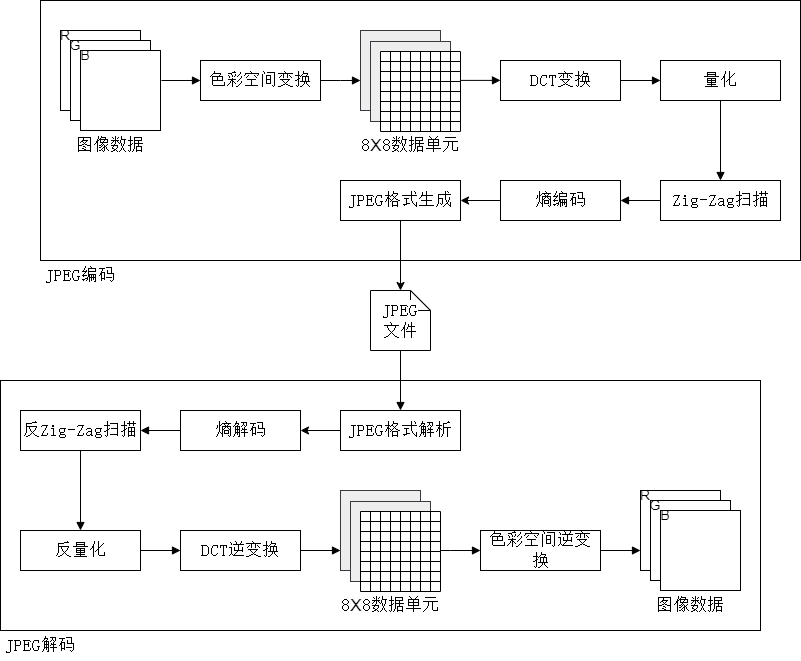
\includegraphics[scale=0.45]{./pictures/编解码流程.png}
    \caption{JPEG的编码和解码流程}\label{jpeg}
  \end{figure}
  JPEG格式的图像压缩流程为:首先将图像每个像素点的R、G、B颜色分量通过色彩空间变
  换转换成色度分量Cr、Cb以及亮度分量Y。之后将图片划分为若干个8*8的数据单元每个
  单元包含64个像素点,再对每个数据单元进行二维离散余弦变换(DCT),将二维的空间
  域数据变成二维的频域数据。再根据量化表对对应的频域分量进行量化处理。再通过Zig-Zag
  扫描将二维的频域数据转换成一维的序列。最后,依次通过游程编码和霍夫曼编码去除掉
  冗余的数据从而压缩JPEG图像数据。

  解压缩流程的流程与压缩的各个流程相反,除了量化和彩色空间变换这一过程会丢失一定
  的信息之外,其他的步骤都可以无损还原原数据,因此JPEG是一种有损压缩技术。

  下面依次对各个步骤做详细的描述。
  \subsection{彩色空间变换及逆变换}
    \vspace{1em}
    绝大多数的颜色都可以使用R、G、B三种颜色分量的线性组合进行合成。因此大多
    图像数据每个像素点都是以RGB分量表示。特别是再计算机视频技术中,不管使用
    哪种形式的彩色空间表示,最后一定要转换为RGB彩色空间显示。

    相关研究表明,人类的视觉系统有分别对红绿蓝三种颜色敏感层度的三种锥体细胞
    以及对明暗程度敏感的锥体细胞。其中对明暗程度的锥体细胞的数量大于对颜色敏
    感层度锥体细胞的数量。因此人类对是对色度辨识度大概是对明暗变换的辨识度的
    四分之一,因此可以利用对颜色感知强度的不同,将RGB彩色空间变换到YCrCb
    \cite{rao2014discrete}彩色空间再根据感知能力做对应的处理。

    ITU-R601建议规定的RGB彩色空间到YCbCr彩色空间变换关系如式(\ref{RGB2YCbCr}):
    \begin{equation}
      \begin{bmatrix}Y\\ Cr\\ Cb\end{bmatrix}=
      \begin{bmatrix}
        0.299 & 0.587 & 0.144\\
        0.500 & -0.419 & -0.081\\
        -0.169 & -0.331 & 0.500
      \end{bmatrix}
      \begin{bmatrix}R\\ G\\ B\end{bmatrix}+
      \begin{bmatrix}0\\ 128\\ 128\end{bmatrix}
      \label{RGB2YCbCr}
    \end{equation}

    在JPEG编码中,RGB颜色分量的取值范围通常是0到255,因此JPEG数据使用的是8位
    无符号整数。而在YCrCb颜色空间中,色度的颜色分量Cr、Cb的范围为-128到127。为
    了将其范围转换为0到255。故添加偏移量128,以确保范围在0到255内。这有助于在
    JPEG编码和解码中正确处理色度信息。这个偏移量是JPEG编码标准的一部分,确保
    了色度信息在JPEG图像中正确显示。

    彩色空间的逆变换如下式所示:
    \begin{equation}
      \begin{bmatrix}R\\ G\\ B\end{bmatrix}=
      \begin{bmatrix}
        1 & 1.402 & 0.\\
        1 & -0.344 & -0.714\\
        1 & 0 & 0.500
      \end{bmatrix}
      \begin{bmatrix}Y\\ Cb\\ Cr\end{bmatrix}+
      \begin{bmatrix}128\\ 128\\ 128\end{bmatrix}
      \label{YCbCr2RGB}
    \end{equation}

    由于人类的视觉系统对色度变化的感知低于亮度,因此在对色度分量进行采样的时
    候可以有选择性地进行降采样,进而降低数据量,这也是最朴素的图像压缩技术之
    一。根据对色度分量的采样率不同分为一下几种采样格式:
     
    YCbCr444:每个分量的采样率都为1。这意味着对于每一个像素点都进行完整的采
    样,携带完整的原图片信息,没有信息丢失。因此YCbCr44也是最高质量的采样格
    式。

    YCbCr422:在每两个水平相邻的像素中,只用一个Cr分量和一个Cb分量来表示该这
    两个像素点的色度分量,而每一个像素点都与之对应的Y分量。这种降采样的方式减
    少了颜色信息的存储和传输需求,在一定程度上牺牲了色度分辨率,但保留了较高
    的图像质量。

    YCbCr420:在每两个水平相邻以及垂直相邻的像素中,只用一个Cr分量和一个Cb分
    量表示这4个像素点的色度分量,而每一个像素点都有一个与之对应的Y分量。这种
    降采样的方式减少了存储和传输的需求,同时牺牲了色度的分辨率,是广泛应用与
    图片和视频压缩的以及传输的一种采样格式。本设计采用该采样格式。

    再经过采样后需要将采样得到的Y、Cb、Cr三种格式分别根据在空间上的分布整合成
    若干个8乘8的数据单元。该数据单元是之后JPEG编解码各个流程之中的处理单位,
    称为MCU(Minimun Coded Unit,最小编码单元)。当使用YCbCr422采样格式时单
    个MCU有2个8乘8的Y分量单元以及Cr和Cb分量8乘8单元各一个。同理,当使用YCbCr
    采样格式时单个MUC有4个8乘8的Y分量单元以及Cr和Cb分量8乘8单元各一个。
  \subsection{离散余弦变换及逆变换}
    \vspace{1em}
    由于人类的视觉系统在对,图像上亮度以及色度在空间上变化频率高的细节部分的注
    意力并不高,因此可以将图像上的高频率的信息适当的过滤掉,进而对数据进行近一
    步的压缩。DCT\cite{ahmed2006discrete}(Discrete Cosine Transform离散余弦变换)
    的作用是将图像从空间域转换到频域。在JPEG中,通过对每个MCU进行2D-DCT从而得到
    在空间上各个频率代表的正交基分量。2D-DCT的变换公式如下:
    \begin{equation}
      \begin{gathered}
        Y(u,v)=\alpha (u)\alpha (v) \sum_{i=0}^{N-1} \sum_{j=0}^{M-1}
        X(i,j)\cos \left[ \frac{\pi}{N}\left(i+\frac{1}{2}\right)u \right]
        \cos \left[ \frac{\pi}{M}\left(j+\frac{1}{2}\right)v \right]\\
        u=0,1,2,\cdots ,N-1 \\
        v=0,1,2,\cdots,M-1 \\
      \end{gathered}
      \label{2D-DCT}
    \end{equation}
    其中
    \begin{equation}
      \alpha (u) = \begin{cases}
        \sqrt{\frac{2}{N}} &,u>0\\
        \frac{1}{\sqrt{N}} &,u=0
      \end{cases}\quad
      \alpha (v) = \begin{cases}
        \sqrt{\frac{2}{M}} &,v>0\\
        \frac{1}{\sqrt{M}} &,v=0
      \end{cases}
    \end{equation}
    在JPEG中对8×8的像素块进行2D-DCT变换,所以有$N=8,M=8$ 。带入(\ref{2D-DCT})有:
    \begin{equation}
      \begin{gathered}
        Y(u,v)=\frac{1}{4}C(u)C(v) \sum_{i=0}^{7} \sum_{j=0}^{7}
        X(i,j)\cos \frac{(2i+1)u\pi}{16}\cos \frac{(2j+1)u\pi}{16}\\
        C (v),C (u) = \begin{cases}
          1 &,u,v>0\\
          \frac{1}{\sqrt{2}} &,u,v=0
        \end{cases}
      \end{gathered}
      \label{8*8 2D-DCT}
    \end{equation}
    在公式中,$f(i,j)$表示在位置$(i,j)$的像素值。其中$F(0,0)$实际上就是对64个像素点做
    加权平均,相当于8×8单元的平均亮度,成为DC(Direct coefficient,直流)系数。其余
    的63个频率值的点称为AC(Alternation coefficient,交流)系数。在交流系数中距离直流
    系数点越大代表该点的频率越高。

    将频域转换成空间域的变换称为IDCT(Inverse Discrete Cosine Transform,离散余弦逆变换)
    ,2D-IDCT的表达式如下:
    \begin{equation}
      \begin{gathered}
        X(i,j)=\frac{1}{4}\alpha(u)\alpha(v)\sum_{u=0}^{7}\sum_{v=0}^{7}
        Y(u,v)\cos\frac{(2i+1)u\pi}{16}\cos\frac{(2j+1)v\pi}{16}\\
          \alpha (v),\alpha (u) = \begin{cases}
            1 &,u,v>0\\
            \frac{1}{\sqrt{2}} &,u,v=0
          \end{cases}
      \end{gathered}
    \end{equation}
  \subsection{量化及反量化}
    \vspace{1em}
    量化是对DCT系数进行压缩的最关键一步,它按照给定的量化系数对每个DCT进行除法,
    再通过四舍五入取整数的方式得到量化后的系数,这个过程是一个一对多的映射过程。
    也就代表量化后的数据将无法完整地还原回来,因此存在数据丢失。这也是导致JPEG有
    损压缩的原因之一,量化的公式如下:
    \begin{equation}
      C(u,v)=round\left[\frac{F(u,v)}{Q(u,v)}\right]
    \end{equation}
    其中$F(u,v)$是2D-DCT系数,$Q(u,v)$是步长值,$C(u,v)$是量化后的值。而反量化
    自然就是将量化后的值乘回步长值,反量化的公式如下
    \begin{equation}
      F(u,v)=C(u,v)Q(u,v)
    \end{equation}

    量化是为了将大部分的高频分量都转换为0,进而减少高频分量的信息,同时也是为了
    下一步编码作出准备。通过不同的量化表从而控制图像的压缩程度。JPEG针对色度以及
    亮度有不同的量化表,如表\ref{亮度量化表}和表\ref{色度量化表}所示

    \begin{table}[H]
      \caption{亮度量化表}
      \label{亮度量化表}
      \centering
      \begin{tabular}{cccccccc}
        \toprule
        \multicolumn{8}{c}{亮度量化表}\\
        \midrule
        16 & 11 & 10 & 16 & 24 & 40 & 51 & 61 \\
        12 & 12 & 14 & 19 & 26 & 58 & 60 & 55 \\
        14 & 13 & 16 & 24 & 40 & 57 & 69 & 56 \\
        14 & 17 & 22 & 29 & 51 & 87 & 80 & 62 \\
        18 & 22 & 37 & 56 & 68 & 109 & 103 & 77 \\
        24 & 35 & 55 & 64 & 81 & 104 & 113 & 92 \\
        49 & 64 & 78 & 87 & 103 & 121 & 120 & 101 \\
        72 & 92 & 95 & 98 & 112 & 100 & 103 & 99 \\
        \bottomrule
      \end{tabular}
    \end{table}

    \begin{table}[H]
      \caption{色度量化表}
      \label{色度量化表}
      \centering
      \begin{tabular}{cccccccc}
        \toprule
        \multicolumn{8}{c}{色度量化表}\\
        \midrule
        17 & 18 & 24 & 47 & 99 & 99 & 99 & 99 \\
        18 & 21 & 26 & 66 & 99 & 99 & 99 & 99 \\
        24 & 26 & 56 & 99 & 99 & 99 & 99 & 99 \\
        47 & 66 & 99 & 99 & 99 & 99 & 99 & 99 \\
        99 & 99 & 99 & 99 & 99 & 99 & 99 & 99 \\
        99 & 99 & 99 & 99 & 99 & 99 & 99 & 99 \\
        99 & 99 & 99 & 99 & 99 & 99 & 99 & 99 \\
        99 & 99 & 99 & 99 & 99 & 99 & 99 & 99 \\
        \bottomrule
      \end{tabular}
    \end{table}

    对比两个表可以明显地看出,对于亮度步长的划分会更细一点,同时高频分量的
    值是普遍大于低频部分的。这是由于人眼对色度和高频部分图像信息的辨识能力
    低于亮度和高频部分。可以把量化当成一个在空间上的二维低通滤波器。
  \subsection{ZigZag扫描及反扫描}
    \vspace{1em}
    \begin{figure}[H]
      \centering
      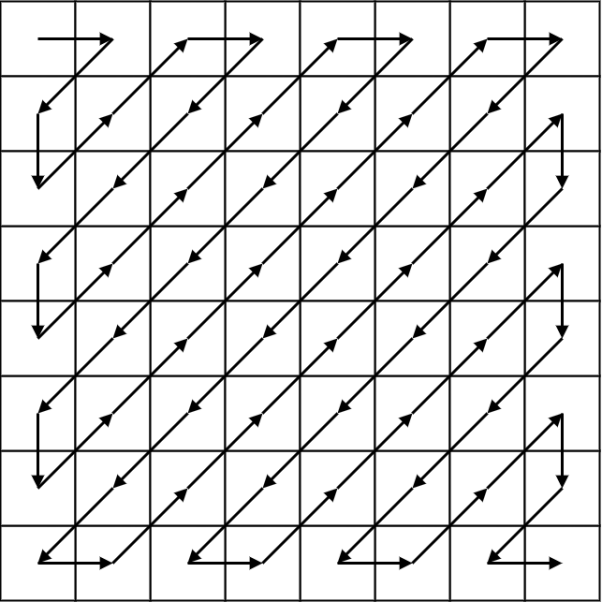
\includegraphics[scale=0.8]{./pictures/zigzag.png}
    \caption{ZigZag扫描}\label{zigzag}
    \end{figure}
    ZigZag扫描的过程如图\ref{zigzag}所示,它对8×8单元进行一维上的重排序。
    这一步骤也可以在量化前执行。对于大部分的8×8单元而言,在经过量化后,右
    下角的高频分量存在大量的零值。为了最大限度地将这些零值相邻为后面压缩做
    准备,通过Z字形扫描对8×8单元进行重排序。同理,反扫描即为将1维序列排回
    8×8单元。
  \subsection{熵编码及熵解码}
    \vspace{1em}
    图像数据的信息冗余量主要体现来两个层面:一是图像数据中各个相邻数据之间
    存在着一定的关联性。在一点体现在空间域上就是相邻的像素点之间的差距一般
    并不是很大,体现在频域上则是在经过量化和ZigZag扫描之后的数据中存在大量
    连续的零值;二是图像中不同的像素值的概率分布通常是不均匀的,某些像素值
    的出现的概率较高。如果对出现概率较高的数据采用跟少的位数进行编码,则能
    在一定程度减少一定的数据量。熵编码的主要目的为通过信息熵理论来减少这些
    冗余的信息,从而降低图像数据在传输和存储中所占用的时间和空间。同时熵编
    码是可逆的属于无失真压缩。

    在量化后。对于DC系数和AC系数两者在统计性质有很大的不同,因此采用两种不
    同的编码方式,对于DC系数采用差分脉冲编码(differential Pluse Code Modulaiton, DPCM)
    ,对于AC系数则使用游程编码(Run-Length Encodeing,RLE)。
    这两种编码方式通过在空间和频率上各个相邻数据的相似性的特点进行编码。在
    霍夫曼编码之前,能有效地减少图像数据的冗余性,以实现更高效的图像压缩。
    \subsubsection{DC系数差分脉冲编码}
    \vspace{1em}
      DC系数的值通常会比AC的值要大,而DC系数可以认为是每个8×8单元的平均值
      。而在空间上相邻的8×8单元平均值的差异通常不大。为了充分利用这一特点
      ,JPEG采用了差分脉冲编码,通过对当前的8×8单元的DC系数与前一个8×8单元
      的DC系数的差值进行编码。设$DC_{diff}$当前的8×8单元的DC系数$DC_{i}$减
      去前一个DC
      系数$DC_{i-1}$,$DC_{0}$表示第一个8×8单元的DC值。公式如下:
      \begin{equation}
        DC_{diff}=\begin{cases}
          DC_{i}-DC_{i-1} &,i>0\\
          DC_{0}&,i=0
        \end{cases}
      \end{equation}

      $DC_{diff}$的编码格式为(Size,Amplitude)。其中Size为Amplitude的位
      宽值,而Amplitude为$DC_{diff}$的幅值,当幅值为正是为原码。反正则为补
      码。因此Amplitude没有符号位。根据Size和Amplitude的第一位来判断
      $DC_{diff}$的正负。
    \subsubsection{AC系数游程编码}
      \vspace{1em}
      在经过ZigZag扫描之后,AC系数通常会出现大量连续的零值。也就可以通过连
      续0的个数来进行编码,这种方式称为游程编码。游程编码可以有效地表示续
      出现的相同的值,用该数值本事加上该数值的重复次数来替代。进而减少数据
      量来做到数据压缩。游程编码的编码格式为(Run,Size,Amplifier)。其中
      Run(游程)表示非零值前面零值的个数,Size表示非零值的尺寸,Amplifier
      表示非零值的幅值。同理,也可以根据这三个值还原回原码,从而做到解码。

      有两种特殊的情况需要注意:当出现从某个非零值直到最后第64个值都为零时
      的情况,使用0/0(EOB)
      进行编码。当连续零值的数量超过16个时,使用F0(ZRL)进行编码。
    \subsubsection{霍夫曼编码}
      \vspace{1em}
      霍夫曼编码是一种可变长度编码,这种编码方法由霍夫曼(Huffman)在1952
      年提出\cite{huffman1952method}。它根据字符的出现的概率来构建编码映射。
      以实现码字的平均长度最短。该编码方式的压缩率接近香农所定义的极限压缩率,
      因此这种方法也称为最佳编码。
      通过查找AC和DC系数对应颜色分量的Huffman表进行编码。Huffman码表是由JPEG
      标准通过大量的图像数据统计进而规定的,详细内容如下表所示。
      \begin{table}[H]
        \centering
        \caption{亮度$DC_{diff}$Huffman表}
        \begin{tabular}{ccc}
          \toprule
          尺寸  & Huffman码长度 & Huffman码字\\
          \midrule
          0     & 2             & 00\\
          1     & 3             & 010\\
          2     & 3             & 011\\
          3     & 3             & 100\\
          4     & 3             & 101\\
          5     & 3             & 110\\
          6     & 4             & 1110\\
          7     & 5             & 11110\\
          8     & 6             & 111110\\
          9     & 7             & 1111110\\
          A     & 8             & 11111110\\
          B     & 9             & 111111110\\
          \bottomrule
        \end{tabular}
      \end{table}

      \begin{table}[H]
        \centering
        \caption{色度$DC_{diff}$Huffman表}
        \begin{tabular}{ccc}
          \toprule
          尺寸  & Huffman码长度 & Huffman码字\\
          \midrule
          0     & 2             & 00\\
          1     & 3             & 010\\
          2     & 3             & 011\\
          3     & 3             & 100\\
          4     & 3             & 101\\
          5     & 3             & 110\\
          6     & 4             & 1110\\
          7     & 5             & 11110\\
          8     & 6             & 111110\\
          9     & 7             & 1111110\\
          A     & 8             & 11111110\\
          B     & 9             & 111111110\\
          \bottomrule
        \end{tabular}
      \end{table}

      \begin{table}[H]
        \centering
        \caption{亮度AC系数Huffman表}
        \begin{tabular}{ccc}
          \toprule
          游程/尺寸 & Huffman码长度 & Huffman码字\\
          \midrule
          0/0(EOB)  & 4             & 1010\\
          0/1       & 2             & 00\\
          0/2       & 2             & 01\\
          0/3       & 3             & 100\\
          0/4       & 4             & 1011\\
          0/5       & 5             & 11010\\
          0/6       & 7             & 1111000\\
          0/7       & 8             & 11111000\\
          0/8       & 10            & 1111110110\\
          0/9       & 16            & 1111111110000010\\
          0/A       & 16            & 1111111110000011\\
          1/1       & 4             & 1100\\
          $\cdots$  & $\cdots$      & $\cdots$\\
          F/A       & 16            & 1111111111111110\\
          \bottomrule
        \end{tabular}
      \end{table}

      \begin{table}[H]
        \centering
        \caption{色度AC系数Huffman表}
        \begin{tabular}{ccc}
          \toprule
          游程/尺寸 & Huffman码长度 & Huffman码字\\
          \midrule
          0/0(EOB)  & 2             & 00\\
          0/1       & 2             & 01\\
          0/2       & 3             & 100\\
          0/3       & 4             & 1010\\
          0/4       & 5             & 11000\\
          0/5       & 5             & 11001\\
          0/6       & 6             & 111000\\
          0/7       & 7             & 1111000\\
          0/8       & 9             & 111110100\\
          0/9       & 10            & 1111110110\\
          0/A       & 12            & 111111110100\\
          1/1       & 4             & 1011\\
          $\cdots$  & $\cdots$      & $\cdots$\\
          F/A       & 16            & 1111111111111110\\
          \bottomrule
        \end{tabular}
      \end{table}

      在解码时,当多个Huffman串行码流排列输出在一起时,可以使用二叉树解索
      引从而获取对应原码从而做到解码得到尺寸,再通过尺寸得到幅值所占的的位
      宽得到幅值。通过这种方式从而区分出码流中的各个像素点的数据。
      \begin{figure}[H]
        \centering
        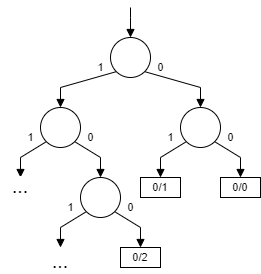
\includegraphics[scale=0.8]{./pictures/deCodeTree.png}
        \caption{通过二叉树解码}
      \end{figure}
  \subsection{JPEG文件格式}
    \vspace{1em}
    通过上述过程得到了压缩之后的图像数据,除此之外,要对数据进行解码。还需
    要知道图像的相关属性等信息。JPEG委员会在指定JPEG标准时,定义了许多用来
    区分图像数据及其相关信息的文件格式。目前,使用比较广泛的是1992年9月由E
    ric Hamilton 提出的JPEG文件交换格式JFIF(JPEG File Interchange Format)
    1.02版本。大多数的设备都支持JFIF文件交换格式。JPEG编码的最后一个步骤就是
    把各种标记代码和编码后的图像数据组成一帧一帧的位码流,这样就方便传输、
    存储和解码器译码。

    JFIF文件格式可以分为两个部分:标识和压缩数据。每个标识的前一个字节是固
    定值0xFF。每个标记之前还可以添加数量不限的0xFF。下表\cite{JFIF}列举几种
    常见的标记码以及它们各自的数据结构。
    \begin{table}[H]
      \centering
      \caption{几种常见的标记}
      \begin{tabular}{cc}
        \toprule
        标记种类 & 含义\\
        \midrule
        SOI & 图像的开始\\
        APP0 & JFIF引用的数据块\\
        SOF0 & 帧开始\\
        DHT & Huffman表\\
        SOS & 扫描线开始\\
        EOI & 图像结束\\
        \bottomrule
      \end{tabular}
    \end{table}
    
    \begin{table}[H]
      \centering
      \caption{APP0标识}
      \begin{tabular}{ccc}
        \toprule
        标识结构 & 字节数 & 含义\\
        \midrule
        0xFF & 1 & \multirow{2}{*}{APP0标识}\\
        0xE0 & 1 &\\
        \bottomrule
      \end{tabular}
    \end{table}

    \begin{table}[H]
      \centering
      \caption{OF0标识}
      \begin{tabular}{ccc}
        \toprule
        标识结构 & 字节数 & 含义\\
        \midrule
        0xFF & 1 & \multirow{2}{*}{APP0标识}\\
        0xC0 & 1 &\\
        $L_{f}$ & 2 & 长度字段,表示图像帧信息长度\\
        P & 1 & 指每个像素点的颜色信息的宽度,通常是8位或12位\\
        Y & 2 & 图像的高度\\
        X & 2 & 图像的宽度\\
        $N_{f}$ & 1 & 图像颜色通道的数量。通常为1或3,分别表示灰度图和RGB彩色图\\
        $N_{NT}$ & 1 & 颜色通道,0表示Y通道,1表示Cb通道,2表示Cr通道\\
        $H_{TN}Y_{TN}$ & 1 & 水平方向和垂直方向的采样率\\
        $T_{QNT}$ & 1 & 表示使用的Huffman编码表的编号\\
        \bottomrule
      \end{tabular}
    \end{table}

    \begin{table}[H]
      \centering
      \caption{DHT标识}
      \begin{tabular}{ccc}
        \toprule
        标识结构 & 字节数 & 含义\\
        \midrule
        0xFF & 1 & \multirow{2}{*}{APP0标识}\\
        0xC4 & 1 &\\
        $L_{b}$ & 2 & 长度字段,表示Huffman码字段的长度\\
        $T_{c}$ & 0.5 & 当为1时,表示使用该表处理AC系数,为0时,表示该表处理DC系数\\
        $T_{b}$ & 0.5 & 表示Huffman表的编号\\
        $L_{i}$ & 1 & Huffman表的长度统计,用于表示不同码字长度的符号数目,i从1到16\\
        $V_{ij}$ & 1 & 代表每一个Huffman码表所代表的值\\
        \bottomrule
      \end{tabular}
    \end{table}

    \begin{table}[H]
      \centering
      \caption{SOS标识}
      \begin{tabular}{ccc}
        \toprule
        标识结构 & 字节数 & 含义\\
        \midrule
        0xFF & 1 & \multirow{2}{*}{APP0标识}\\
        0xDA & 1 &\\
        $L_{s}$ & 2 & 长度字段,表示数据内容的长度\\
        $N_{s}$ & 1 & 表示扫描所涉及到颜色通道的数量\\
        $C_{s}N_{s}$ & 0.5 & 表示Scan中成分的编号\\
        $T_{d}N_{s}$,$T_{a}N_{s}$ & 1 & $T_{a}N_{s}$表示数据的高4位$T_{a}N_{s}$表示数据的低4位\\
        $S_{s}$ & 1 & 一般为0\\
        $S_{s}$ & 1 & 一般为63\\
        $A_{b}$,$A_{l}$ & 1 & 一般为0\\
        \bottomrule
      \end{tabular}
    \end{table}

    \begin{table}[H]
      \centering
      \caption{EOI标识}
      \begin{tabular}{ccc}
        \toprule
        标识结构 & 字节数 & 含义\\
        \midrule
        0xFF & 1 & \multirow{2}{*}{EOI标识}\\
        0xD9 & 1 &\\
        \bottomrule
      \end{tabular}
    \end{table}
  \subsection{本章总结}
    \vspace{1em}
    本章阐述了JPEG图像数据编解码的原理和相关理论,JPEG图像压缩技术通过一系列
    高效的步骤,在保证视觉质量的同时显著地减少数据量。其核心思想是利用人眼的
    感知特性,通过色度下降采样减低冗余信息,再结合离散余弦变换将将图像从空间
    域转换到频域,通过量化将能量集中在低频部分,并且量化阶段通过牺牲高频细节
    进一步压缩数据。而Zigzag扫描和熵编码则有效地减少了数据中统计冗余。最终,
    压缩后的数据通过JFIF文件格式进行组织存储。

\newpage
\section{JPEG编码系统硬件结构设计}
  \vspace{1em}
  上一章节讲解了JPEG编码的步骤和过程。这一章讲解本设计如何使用硬件实现JPEG
  的编码以及解码。内容包含数字电路设计中的一些设计思想\cite{2004vlsi数字信号处理系统}
  ,编码系统的结构划分,以及各个模块的结构和运行原理。
  \subsection{设计思想}
    \vspace{1em}
    在数字系统设计中,一个经常围绕的问题就是速度和面积的权衡。使用多个处理
    单元对数据进行处理是一种朴素的提高系统计算速度和吞吐量的方式。与之带来
    的副作用就是电路面积的增大。面积增大所带来的副作用不仅仅是成本增加的问
    题,它也伴随着系统功耗和发热量的增加,这些负面影响都会降低系统的稳定性
    。而有些运算过程数据依赖性高、并行操作无法有效地提高性能。甚至可能因为
    额外的开销导致性能的下降。因此,一个好的数字系统设计往往能够权衡速度和
    面积。

    通过前人的大量经验实践总结出了大量的设计思想。如果能在合适的情况下使用
    这些设计思想,就能得到一个好的设计。下面描述变设计所使用的几种设计思想
    。
    \subsubsection{流水线}
      \vspace{1em}
      如果一个运行周期长的操作的运行过程能个分解成一各个子步骤。并将这些子
      步骤封装成一个个并行的模块。让每个操作的不同步骤在不同时刻错开运行,
      每个模块同时执行不同操作所对应的步骤。最终每经过一个子步骤的时间,就
      可以得到一个操作的运行结果,通过这种方式系统的吞吐量能得到大幅度提高
      ,在运行过程中每个步骤的结果数据一步步的从输入流动到输出,因此该操作
      得名流水线(Pilpeline)。这种方式在如今的工厂车间运用广泛。

      下面通过对比一个分3个步骤的执行的例子,来分析流水线所带来的性能的提
      升。假设一个系统的执行需要通过步骤一、步骤二、步骤三三个步骤的到结果,
      每个步骤所花费的时间为一个时钟周期。如果依次按照顺序完成N次运算,每
      隔3个时钟周期得到一个运行结果,完成所有运算所花费的时间就是3N。如果
      设置三个执行不同步骤的模块同时并行执行,且每个模块执行不同操作的步骤
      ,如第一个时刻执行步骤一的模块执行操作一的步骤一,如第二个时刻执行步
      骤一的模块执行操作二的步骤一,执行步骤二的模块执行操作一的步骤二;第
      三个时刻执行步骤一的模块执行操作三的步骤一,执行步骤二的模块执行操作
      二的步骤二,执行步骤三的模块执行操作一的步骤三;之后N个时刻以此类推
      在第4个时刻得到操作一的结果,下一时刻得到操作二的结果。之后每经过一
      个时刻得到一个操作结果。得到N操作的结构则需要花费3+N个时钟周期的时间
      。通过这种方式显著地提升数据的吞吐量。
      \begin{figure}[H]
        \centering
        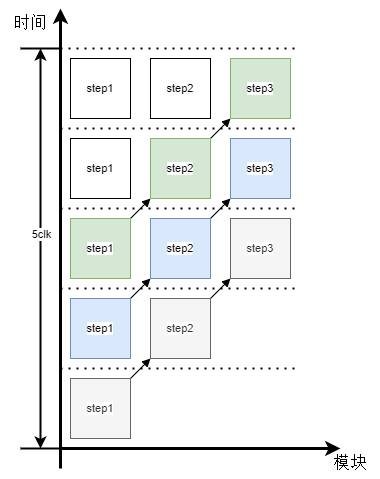
\includegraphics[scale=0.6]{./pictures/流水线.png}
        \caption{流水线操作}
      \end{figure}

      除此之外,流水线通常用于提高数字电路的最大运行时钟频率。在时序电路中
      时钟周期至少要大于保持时间、建立时间、组合逻辑延迟时间三者之和。而组
      合逻辑延迟时间取决于组合逻辑中最长的电路路径。如果在组合逻辑之中插入
      寄存器,从而切分组合逻辑的关键路径,使组合逻辑在每个时钟周期安装流水
      线的方式运行。通过这种方式提高时序电路的最大运行时钟频率。从而提高整
      个电路的运算速度。
      \subsubsection{脉动阵列}
        \vspace{1em}
        脉动阵列(Systolic Array)是一种由众多简单的运算元件(Processing 
        Element,PE)按照一定的规则排列的硬件架构。它最早由H.T.
        Kung在1982年提出\cite{kung1982systolic}。一个脉动阵列具备一下特征
        \cite{2004vlsi数字信号处理系统}:

        (1)由单一或多种构造的PE按照规则排列;

        (2)只有相邻的PE互相连接,数据只能通过在局部范围内移动;

        (3)PE只重复进行简单的数据处理和必要的数据收发;

        (4)所有PE由统一的时钟同步工作;

        每个PE都和相领的PE同步进行数据收发和运算。数据从外部流入,PE阵列一
        边搬运数据,一边采用流水线或并行的方式对其进行处理。各个PE的运算和
        数据的收发动作和心脏规律地收缩促使血液流动的过程非常相似,因此得称
        脉动阵列。

        由于脉动阵列的数据移动只在相邻的PE中进行,这种方式有利于芯片或FPGA
        的布局步线,脉动阵列根据排列和连接方式,主要可分为串行的一维脉动阵
        列,网格连接的二维脉动阵列。其中一维的脉动阵列能实现FIR滤波器,向
        量乘法,数据排序。二维脉动阵列能完成矩阵运算,如图\ref{2D array}。
        \begin{figure}[H]
          \centering
          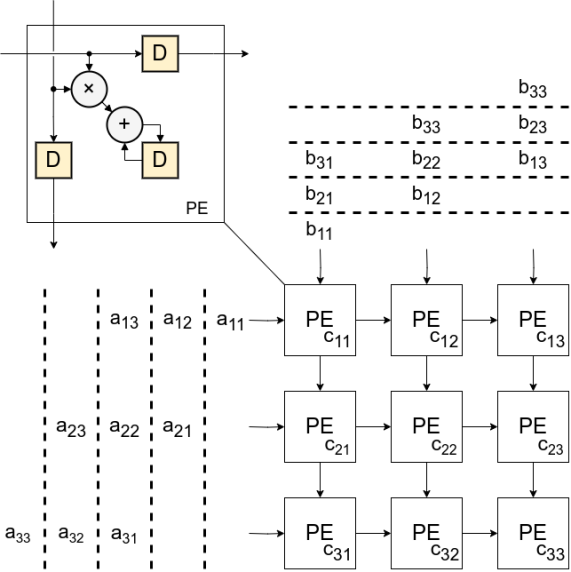
\includegraphics[scale=1]{./pictures/2Darray.png}
          \caption{二维脉动技术矩阵乘法}
          \label{2D array}
        \end{figure}

        \subsubsection{乒乓操作}
          \vspace{1em}
          在两个功能模块进行数据传输时,如果两个模块的吞吐量不同,对数据接
          收的顺序存在差异等原因。导致两个模块不能够同时工作。这个情况下就
          可以在两个模块之间添加乒乓缓存(Ping-pong 
          buffer)来解决这个问题,这种解决方法被称为乒乓操作。

          乒乓操作的处理流程,在两个模块之间添加2个buffer,来进行缓存数据
          。这个buffer通常是FIFO(First in first 
          out,先入先出队列)或者RAM。初始状态下,数据发送模块先向一个buff
          er写入发送的数据,当buffer的容量满后,数据接收模块开始向这个buff
          er读出数据。同时数据模块继续向另外一个buffer进行写入。之后依次类
          推,两个buffer交错读写。这样,只有在初始时数据发送模块在往第一个
          buffer写入数据时,接收模块是空闲状态,在其余时间内,两个模块都是
          同时工作的。
          \begin{figure}[H]
            \centering
            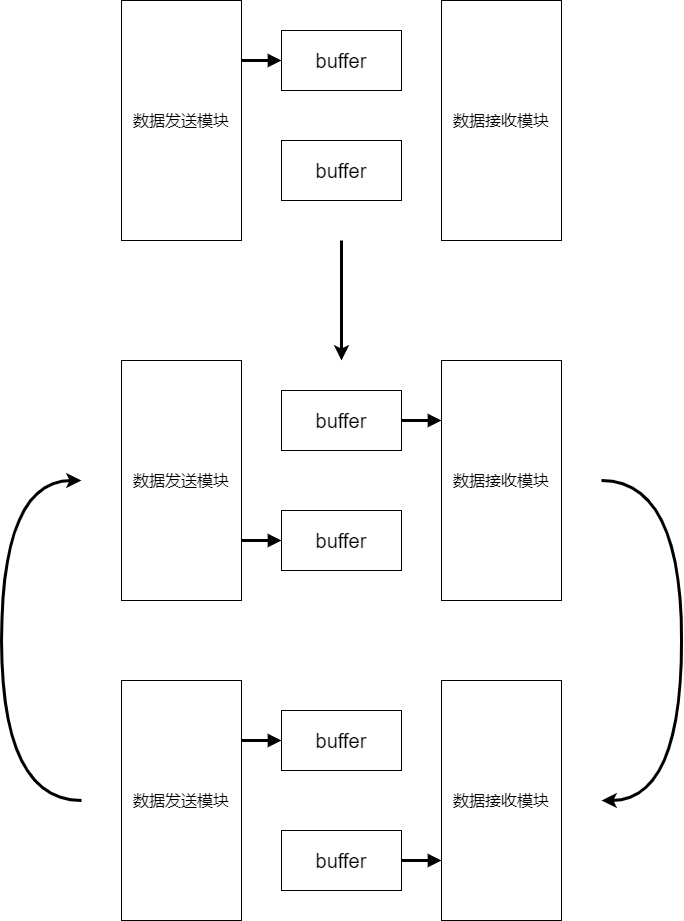
\includegraphics[scale=0.3]{./pictures/乒乓操作.png}
            \caption{乒乓操作}
            \label{2D array}
          \end{figure}

        \subsubsection{算法状态机}
          \vspace{1em}
          在数字系统中,逻辑设计可分为两类。一类是设计执行数据处理的电路,称为
          数据通路。另一类是设计控制不同指令执行循序的电路,称为控制通路。控制
          通路和数据通路的连接关系如图\ref{asmd}所示。数据通路根据系统的功能对
          寄存器进行操作,控制单元为数据通路提供一些系列控制信号。需要注意,从
          数据通路到控制单元的反馈为系统的稳定性提供了保证。
          \begin{figure}[H]
            \centering
            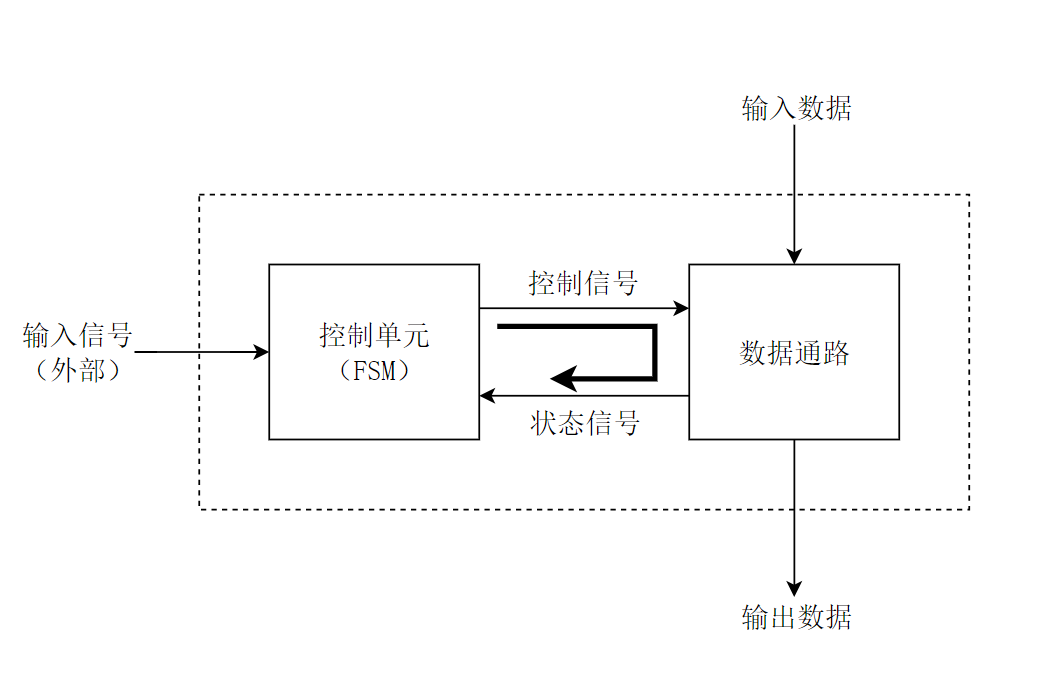
\includegraphics[scale=0.4]{./pictures/ASMD.png}
            \caption{控制单元以及数据通路}
            \label{asmd}
          \end{figure}
          在一般情况下控制单位使用FSM来实现。它能产生控制数据通路的时序信号。FSM
          的次态逻辑取决于当前状态、外部输入和数据通路的状态。在状态转移时会引起
          操作。

          利用流程图可以很便捷地表示步骤和以及算法的判决。硬件算法的流程图将字面
          描述翻译成图中的信息。使用一系列的操作和必要的条件实现。本文采用一种特
          殊的流程图定义数字硬件算法,称之为算法状态机(ASM)。ASM流程图与传统的
          流程图类似,但是在解释的时候有一些不同。传统的流程图以顺序的方式描述步
          骤和算法的关系,但是没有考虑数字电路中的时序关系。ASM流程图描述的是顺
          序事件、时序控制电路的状态与状态转移时发生的时序关系(例如事件随着状态
          的改变而发生同步变化)。在数字系统中,指定准确的时序和数据路径是非常重
          要的,同时要考虑对数字硬件的约束。

          \begin{figure}[H]
            \centering
            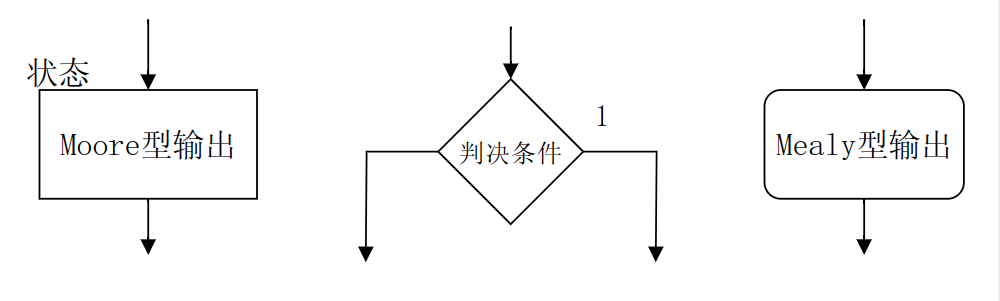
\includegraphics[scale=0.4]{./pictures/ASM构成.png}
            \caption{ASM图的构成}
            \label{asm}
          \end{figure}

          ASM图由三个部分组成,如图\ref{asm}从左到有依次是状态框、判决框和条件框。
          各个框之间有直线连接在一起,表示执行的先后顺序和当前工作顺序和状态机工作
          时发生的状态变化。下面依次介绍这三个部分。

          状态框表示FSM运行时的一个状态,状态框的形状为矩形,在左上角标注有该状态
          的名称。由于Moore型的输出只与当前状态有关,所以矩形框里面标注有此状态下
          的Moore性输出,表示该信号使能。没有标注在该状态框下的moore性信号则不使能。

          判决框描述了输入信号对控制系统的作用。这些输入可以是外部输入,也可以是
          数据通路的状态信息。判决框的形状为菱形框,带有2个退出路径。测试输入的条件
          写在框内,选择哪条退出路径退出判决框,要取决与条件的判决。在二进制系统中
          如果条件为真,将从一条退出路径退出,否则则从另一条退出路径退出。两条路径
          分别用1(TURE)和0(FALSE)表示。为了流程图的简洁,本文只标出了1,未标记
          的路径则为0。

          ASM流程图的状态框和判决框与传统的流程图类似。二条件框是ASM流程图所特有的
          。条件框的形状为圆角矩形。条件框里面的输出信号为Mealy型输出,输出不仅与
          状态有关,还与输入有关。所以条件框的输入路径一定是来自判决框的输出路径。

          \begin{figure}[H]
            \centering
            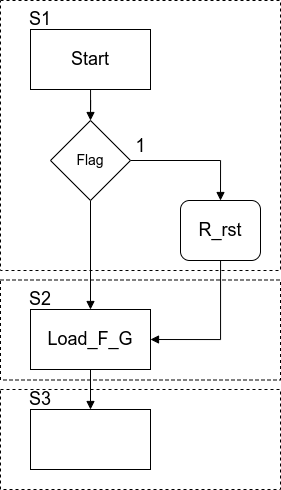
\includegraphics[scale=0.6]{./pictures/ASM_exp.png}
            \caption{ASM的实例}
            \label{asm exp}
          \end{figure}
          
          图\ref{asm exp}为ASM流程图的一个例子。当控制逻辑单元处于状态S1时,产生Start
          输出信号。同时控制单元检查输入Flag是否有效,如果Flag有效则控制单元输出R\_rst
          有效,使寄存器R复位,否则R保持不变。在这两种情况下,次态都为S2。寄存器操作
          与S2有关。但是注意到,这样的表示会导致一些疑惑,因为在FSM在S1状态下并不执行
          寄存器操作R<=0,在状态S2时也不执行操作F<=G。这种表示法其实暗示了当控制单元
          处于S1时,只有Mealy型输入信号有效,才能执行数据路径单元里的操作R<=0,这是由
          与Flag=1确定的,类似地,在状态S2时,只有满足输入条件,数据通路里的寄存器操作
          R<=G才会被执行。数据通路的操作是与时钟是同步的。这个时钟边沿引起状态S1跳转
          到S2,再相应地从S2跳转到S3。此时,在给定状态下产生的控制信号会在下一个时钟
          上升边沿到来时影响寄存器的操作,操作的结果在次态中才能显现出来。
          
  \subsection{编码模块划分}
    \vspace{1em}
    \begin{figure}[H]
      \centering
      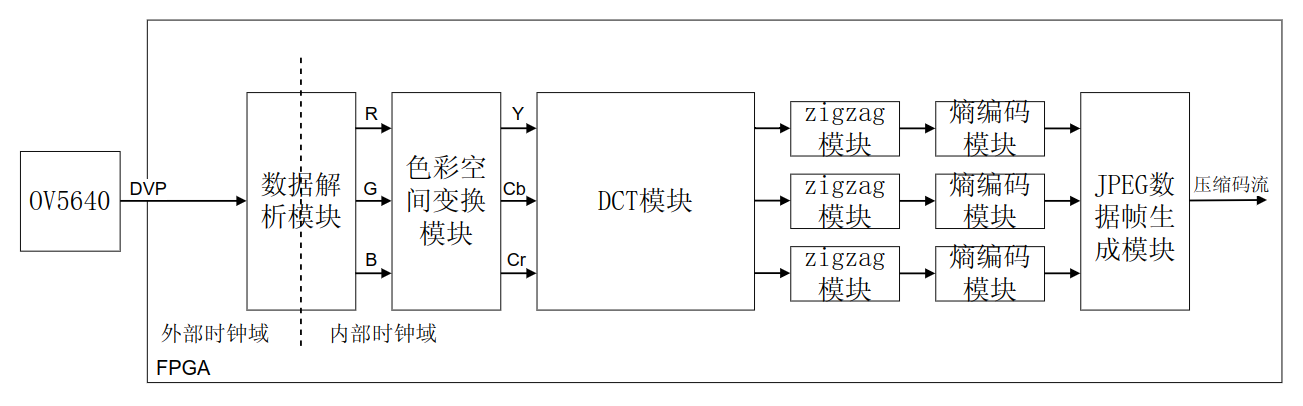
\includegraphics[scale=0.3]{./pictures/CoderTop.png}
      \caption{编码模块}
      \label{code module}
    \end{figure}
    \begin{figure}[H]
      \centering
      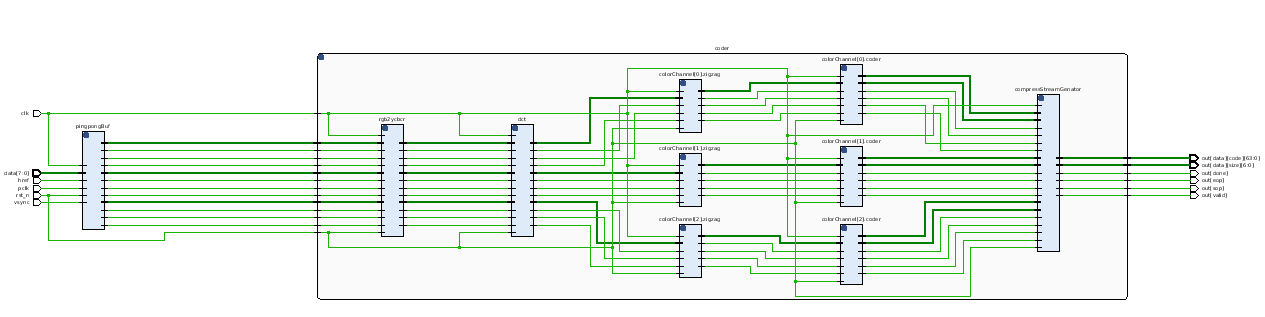
\includegraphics[scale=0.3]{./pictures/TOPrtl.png}
      \caption{编码模块rtl视图}
      \label{code module rtl}
    \end{figure}
    JPEG编码模块的内部模块划分如图\ref{code 
    module},它接收从外部输入进来的RGB格式的图像数据。输出jpeg格式的
    压缩码流。视频信号依次经过数据解析模块、色彩空间变换模块、DCT模块、熵编码
    模块、JPEG数据帧生成模块。使用vivado实际RTL综合后的RTL视图如图\ref{code module rtl}
    所示,可以看出其中各个模块的输入输出接口都包含data、valid、sop、eop四种个信号。
    该信号的功能描述如表\ref{模块输入输出接口}所示。

    \begin{table}[H]
      \centering
      \caption{模块输入输出接口}
      \begin{tabular}{ccc}
        \toprule
        信号名称 & 宽度 & 功能\\
        \midrule
        data & 由数据种类决定 & 传输并处理的数据\\
        valid & 1 & 有效时表示此时数据有效\\
        sop & 1 & 帧头信号,当数据为图像帧的第一个数据时有效\\
        eop & 1 & 帧尾信号,当数据为图像帧的最后一个数据时有效\\
        \bottomrule
      \end{tabular}
    \end{table}

    数据解析模块对其进行跨时域乒乓,并将其转换为后续模块处理的每个颜色通道的8×8
    数据单元;色彩空间模块将RGB格式的信号转换为YCbCr格式的颜色分量;DCT模块对每
    个颜色通道的8×8单元进行2D-DCT;zigzag模块对8×8单元进行zigzag扫描以及量化,熵
    编码模块对其进行编码压缩,JPEG数据生成模块对多个颜色通道的压缩模块进行拼接并
    且添加JPEG文件格式的关键帧;下面的小节详细介绍这4个模块。
  \subsection{数据解析模块}
    \vspace{1em}
    数据解析模块对输入的图像数据进行缓存,由于后续模块输入的数据是以8×8单元作为单位
    依次输入处理的。所以需要对输入的信号进行重排序。本设计采用乒乓操作的方式对输入
    数据进行缓存。再将其进行缓存排序得到符合DCT模块8×8像素单元输入的信号。数据解析
    模块的结构如图\ref{data parser}。
    \begin{figure}[H]
      \centering
      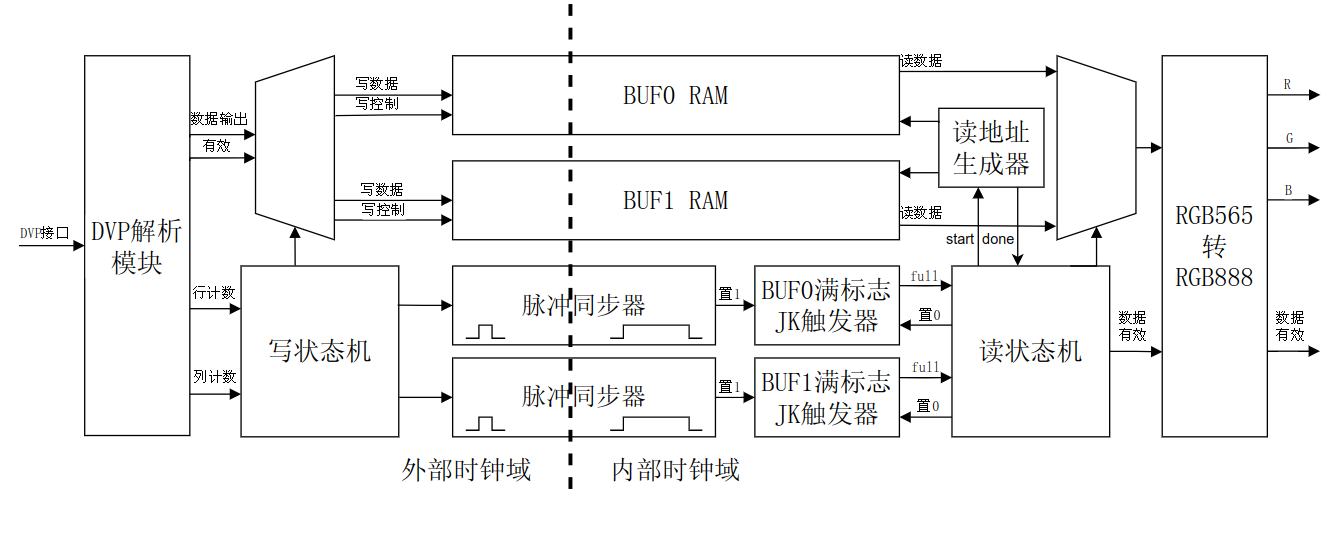
\includegraphics[scale=0.35]{./pictures/数据解析模块.png}
      \caption{数据解析模块结构图}
      \label{data parser}
    \end{figure}

    由于输入的图像RGB数据是以水平扫描的方式顺序进行输出的。所以要以8×8单元的顺序进行输
    出就要先缓存8行数据。再进行读取输出,本设计采用乒乓操作的方式对数据进行缓存输出,
    确保输出数据和输入数据的吞吐量能保持一致。写缓存部分的电路和读缓存部分的电路工作
    在不同的时钟域下。写缓存部分的电路使用模块输入数据的作为时钟输入。读缓存部分的时钟
    采用FPGA内部PLL生成的时钟信号。

      \subsubsection{写状态机以及读状态机}
      写状态和读状态机分别控制写缓存和读缓存从而进行乒乓操作。它们都拥有BUF0
      和BUF1两个状态分别代表对当前对应的BUF进行读写操作。
      写状态机的ASM图如图\ref{wrASM}所示。
      \begin{figure}[H]
        \centering
        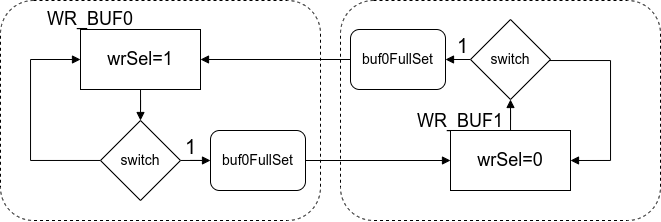
\includegraphics[scale=0.45]{./pictures/wrASM.png}
        \caption{写入状态机ASM图}
        \label{wrASM}
      \end{figure}
      当行计数和列计数的值满足8行时,switch信号有效。同时对于BUF置位满信号。
      接着跳转到另一个BUF所对应的状态。

      读出状态机的ASM图如图\ref{rdASM}所示。
      \begin{figure}[H]
        \centering
        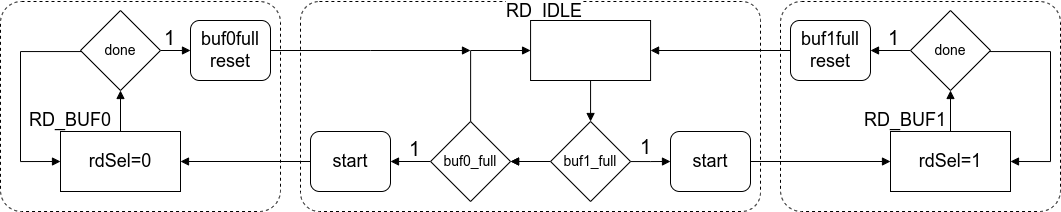
\includegraphics[scale=0.45]{./pictures/rdASM.png}
        \caption{读出状态机ASM图}
        \label{rdASM}
      \end{figure}
      在RD\_IDLE状态下检查2个BUF的full标志位,如果对应的标志位有效则跳转到对应
      BUF的状态,在RD\_BUF1满信号的优先级比RD\_BUF0的满信号高。同时启动读地址
      生成器的start信号,在对应的RD\_BUF检测地址生成器完成的done信号。当done
      有效时就跳转回RD\_IDLE状态,同时使能对应BUF满标志位的置零信号,将其置0。

      由于写状态机和读状态机都工作在不同的时钟域下,所以满标志位JK寄存器的置1
      信号需要通过脉冲同步器进行跨时域传输。脉冲同步器的内部结构如图
      \ref{pulse synchronizer}所示。
      \begin{figure}[H]
        \centering
        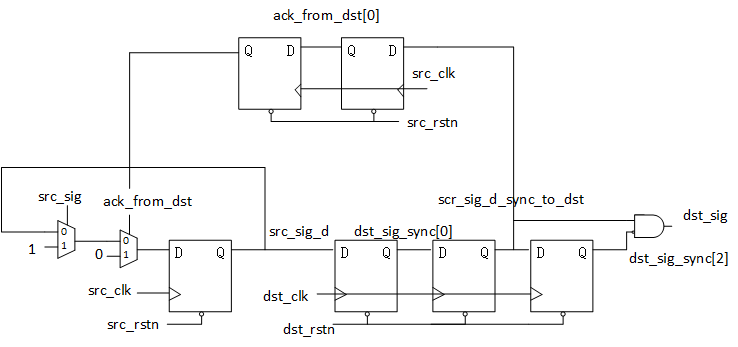
\includegraphics[scale=0.45]{./pictures/脉冲同步器.png}
        \caption{脉冲同步器}
        \label{pulse synchronizer}
      \end{figure}
      脉冲同步器将一个时钟域发出的窄脉冲信号传输到另一个时钟域,同时保证在另一
      个时钟域。在空闲状态下所有D触发器的输出都为0。脉冲输入信号src\_sig拉高时,
      由于mux的选择信号ack\_from\_dst初态为0。所以此时构成一个正反馈使src\_sig\_d
      保持为1。进而使src\_sig\_d的1能同步目的时钟域src\_sig\_sync\_to\_dst信号,
      ,再通过ack\_from\_dst反馈回ack\_from\_dst构成负反馈,使src\_sig\_d保持回
      0。当高电平传输到src\_sig\_sync\_to\_dst时,通过延迟一拍取非再与次态相与捕捉
      其上升沿,得到目的时钟域的窄脉冲信号。在单bit信号跨时钟域传输时为了防止出现
      亚稳态,需要同dst\_sig\_sync以及ack\_from\_dst一样延迟两拍进行传输。

  \subsection{色彩空间变换模块}
    色彩空间变换模块,将RGB颜色空间转换为YCrCb颜色空间。由式(\ref{RGB2YCbCr})可知,
    对于Y颜色分量其中为R、G、B三个颜色分量的乘积和。因此可以使用图\ref{tree}。所示
    的树性流水线的得到变换结果。
    \begin{figure}[H]
      \centering
      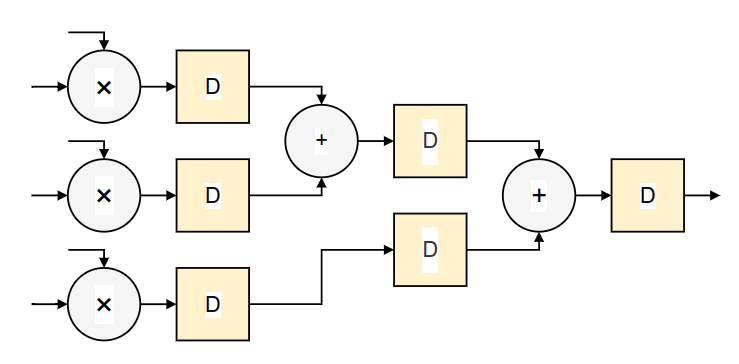
\includegraphics[scale=0.5]{./pictures/彩色空间转换模块.png}
      \caption{树形计算结构}
      \label{tree}
    \end{figure}
    对于其他2个分量也是如此,不同之处在于。色度分量还需加上常数128来得到结果。

  \subsection{DCT模块}
    \vspace{1em}
    DCT模块接收数据预处理模块输出的,Y、Cr、Cb三个颜色通道的8*
    8像素单元。并对每个颜色通道实现进行DCT、量化、Zigzag扫描这三个步骤。
    \begin{figure}[H]
      \centering
      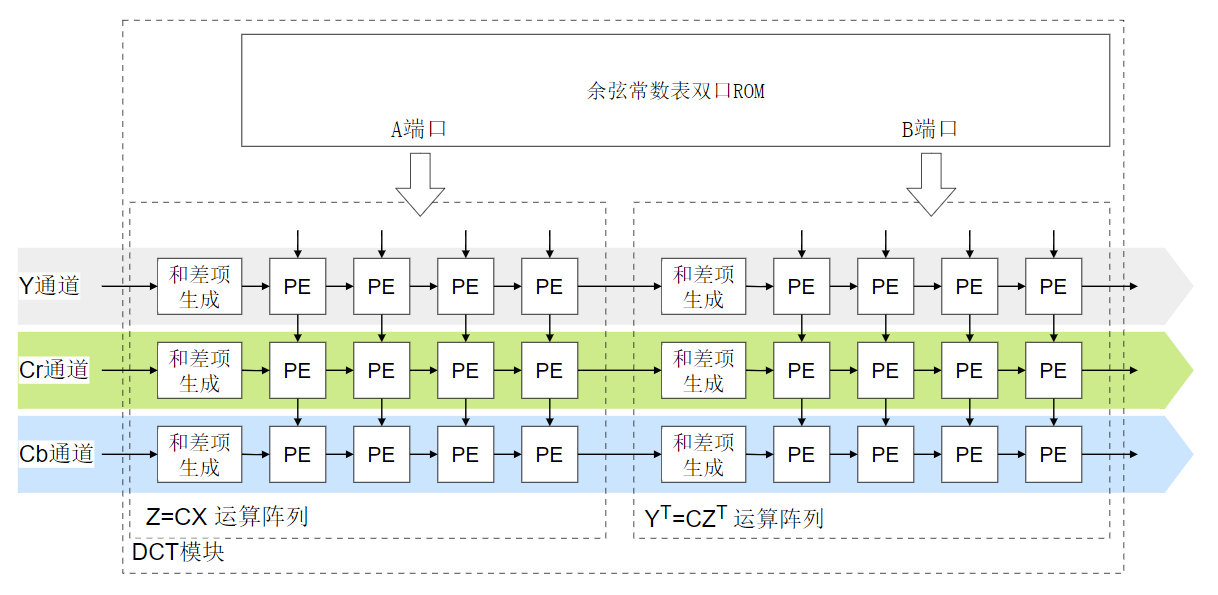
\includegraphics[scale=0.5]{./pictures/dct.png}
      \caption{DCT模块内部结构}
      \label{code module}
    \end{figure}

    如果采用YCrCb444以外的采样格式,则Cr、Cb可以复用一个通道,减少资源的消耗。
    
    根据2D-
    DCT原公式(\ref{8*8 2D-DCT}),对单个8×8单元进行运算,需要进行4096次乘法和40
    96次加法加法运算。需要使用较多的大量的乘法器资源,而乘法器资源在fpga中比较
    稀缺。为了降低计算的复杂度,本设计使用了DA算法\cite{chen1977fast},通过行列分解2D-DCT运算。
      \subsubsection{DA算法}
        \vspace{1em}
        根据式(\ref{8*8 2D-DCT})的特征可以根据行和列分解成两次一维的DCT变换,
        计算过程如下:
        \begin{equation*}
          \begin{aligned}
            Y(u,v)&=\frac{1}{4}C(u)C(v)\sum_{i=0}^{7}\sum_{j=0}^{7}X(i,j)
            \cos\frac{(2i+1)u\pi}{16}\cos\frac{(2j+1)v\pi}{16}\\
            Y(u,v)&=\frac{1}{2}C(u)\sum_{i=0}^{7}\cos\frac{(2i+1)u\pi}{16}
            \frac{1}{2}C(v)\sum_{j=0}^{7}X(i,j)\cos\frac{(2j+1)v\pi}{16}
          \end{aligned}
        \end{equation*}
        令
        \begin{equation}
          Z(i,v)=\frac{1}{2}C(v)\sum_{j=0}^{7}X(i,j)\cos\frac{(2j+1)v\pi}{16}
          \label{colDCT}
        \end{equation}
        有
        \begin{equation} 
          Y(u,v)=\frac{1}{2}C(u)\sum_{i=0}^{7}
          Z(i,v)\cos\frac{(2i+1)u\pi}{16}
          \label{rowDCT}
        \end{equation}

        下面再将式(\ref{colDCT})和式(\ref{rowDCT})整理成矩阵运算,令$C$为带
        常数项的系数矩阵,则有
        \begin{equation}
          C=\begin{bmatrix}
            a & a   & a   & a   & a   & a   & a   & a\\
            b & d   & e   & g   & -g  & -e  & -d  & -b\\
            c & f   & -f  & -c  & -c  & -f  & f   & c\\
            d & -g  & -b  & -e  & e   & b   & g   & -d\\
            a & -a  & -a  & a   & a   & -a  & -a  & a\\
            e & -b  & g   & d   & -d  & -g  & b   & -e\\
            f & -c  & c   & -f  & -f  & c   & -c  & f\\
            g & -e  & d   & -b  & b   & -d  & e   & -g\\
          \end{bmatrix},
          \begin{bmatrix}
            a \\ b \\ c \\ d \\ e \\ f \\ g
          \end{bmatrix}=
          \frac{1}{2}\begin{bmatrix}
            \cos(4\pi/16)\\
            \cos(\pi/16)\\
            \cos(2\pi/16)\\
            \cos(3\pi/16)\\
            \cos(4\pi/16)\\
            \cos(5\pi/16)\\
            \cos(6\pi/16)\\
          \end{bmatrix}
          \label{C}
        \end{equation}
        则式(\ref{colDCT})和式(\ref{rowDCT})的矩阵形式分别为
        \begin{equation}
          Z=CX 
          \label{col}
        \end{equation}
        \begin{equation}
          Y=(CZ^{T})^{T}
        \end{equation}
        整理得
        \begin{equation}
          Y^{T}=C(CX)^{T} 
          \label{rowColDCT}
        \end{equation}
        通过上述步骤,将8×8的2D-DCT分解成两次对$C$的左乘运算。对于Z的每个列
        向量有
        \begin{equation}
          \begin{bmatrix}
            z_{i0}\\z_{i1}\\z_{i22}\\z_{i3}\\z_{i4}\\z_{i5}\\z_{i6}\\z_{i7}
          \end{bmatrix}=\begin{bmatrix}
            a & a   & a   & a   & a   & a   & a   & a\\
            b & d   & e   & g   & -g  & -e  & -d  & -b\\
            c & f   & -f  & -c  & -c  & -f  & f   & c\\
            d & -g  & -b  & -e  & e   & b   & g   & -d\\
            a & -a  & -a  & a   & a   & -a  & -a  & a\\
            e & -b  & g   & d   & -d  & -g  & b   & -e\\
            f & -c  & c   & -f  & -f  & c   & -c  & f\\
            g & -e  & d   & -b  & b   & -d  & e   & -g\\
          \end{bmatrix}\begin{bmatrix}
            x_{i0}\\x_{i1}\\x_{i22}\\x_{i3}\\x_{i4}\\x_{i5}\\x_{i6}\\x_{i7}
          \end{bmatrix}
          \label{colDCTCol}
        \end{equation}
        观察到$C$具有左右对称的性质,可将(\ref{colDCTCol})分解如下
        \begin{equation}
          \begin{bmatrix}
            z_{i0}\\z_{i2}\\z_{i4}\\z_{i6}\\
          \end{bmatrix}=\begin{bmatrix}
            a & a   & a   & a\\
            c & f   & -f  & -c\\
            a & -a  & -a  & a\\
            f & -c  & c   & -f\\
          \end{bmatrix}\begin{bmatrix}
            x_{i0}+x_{i7}\\
            x_{i1}+x_{i6}\\
            x_{i2}+x_{i5}\\
            x_{i3}+x_{i4}\\
          \end{bmatrix}, 
          \begin{bmatrix}
            z_{i1}\\z_{i3}\\z_{i5}\\z_{i7}\\
          \end{bmatrix}=\begin{bmatrix}
            b & d   & e   & g\\
            d & -g  & -b  & -e\\
            e & -b  & g   & d\\
            g & -e  & d   & -b\\
          \end{bmatrix}\begin{bmatrix}
            x_{i0}-x_{i7}\\
            x_{i1}-x_{i6}\\
            x_{i2}-x_{i5}\\
            x_{i3}-x_{i4}\\
          \end{bmatrix}
        \end{equation}
        $Z$每个列向量的偶项等于$x_{n}+x_{7-n}$(下面统称为和项)的线性组合,
        奇项等于$x_{n}-x_{7-n}$的线性组合。对于$Y^{T}=CZ^{T}$也是同理。

        通过上述步骤将8乘8的矩阵运算转换为两次4乘4的矩阵运算。减少了计算的复
        杂度减少了一倍。为了在硬件中使用定点数运算,将中各个系数都扩大$2^{10}$倍,
        相当于将系数左移10位,再将输出的乘积右移进行截位得到结果。

      \subsubsection{DA算法的硬件实现}
        \vspace{1em}
        对于DA算法中2次4乘以4的矩阵运算,本文提出了一种基于脉动阵列的硬件实
        现。 如图\ref{code module}所示。对于单个颜色通道,可以认为一维脉动阵列
        如图\ref{code module}为单个颜色通道计算$Z=CX$的结构。图\ref{code module}
        中输入以$x_{00},x_{07},x_{01},x_{06},x_{02},x_{05},x_{03},x_{04}$的顺序依次输入
        到和差项生成模块生成$x_{00}+x_{07},x_{00}-x_{07}$到$x_{03}-x_{04},x_{03}+x_{04}$,
        的和差项。再将和差项送进一行四列的脉动阵列。得到$z_{00}$到$z_{07}$。
        \begin{figure}[H]
          \centering
          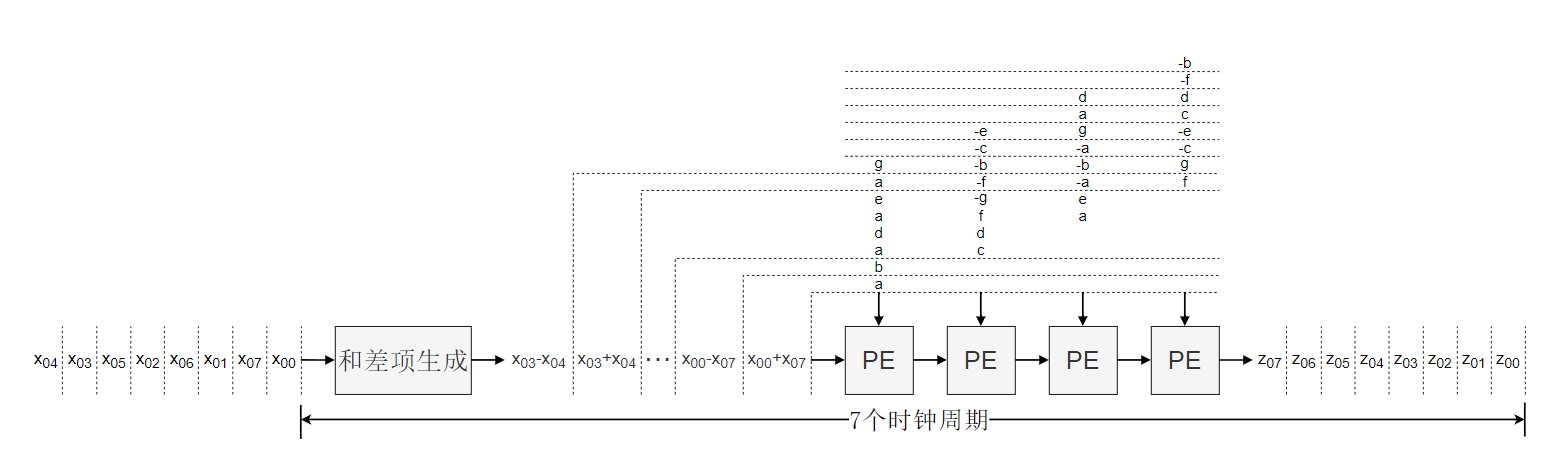
\includegraphics[scale=0.425]{./pictures/DCT脉动阵列.png}
          \caption{计算$Z=CX$的一维脉动阵列实现}
          \label{DCT脉动阵列}
        \end{figure}
        计算$Z=CX$和$Y^{T}=CZ^{T}$,脉动阵列的原理一致,区别在于内部移位寄存器
        延迟的时钟周期数不同,两个矩阵运算的PE内部构成如图\ref{x2zPE}和图\ref{z2yPE}
        所示
        \begin{figure}[H]
          \centering
          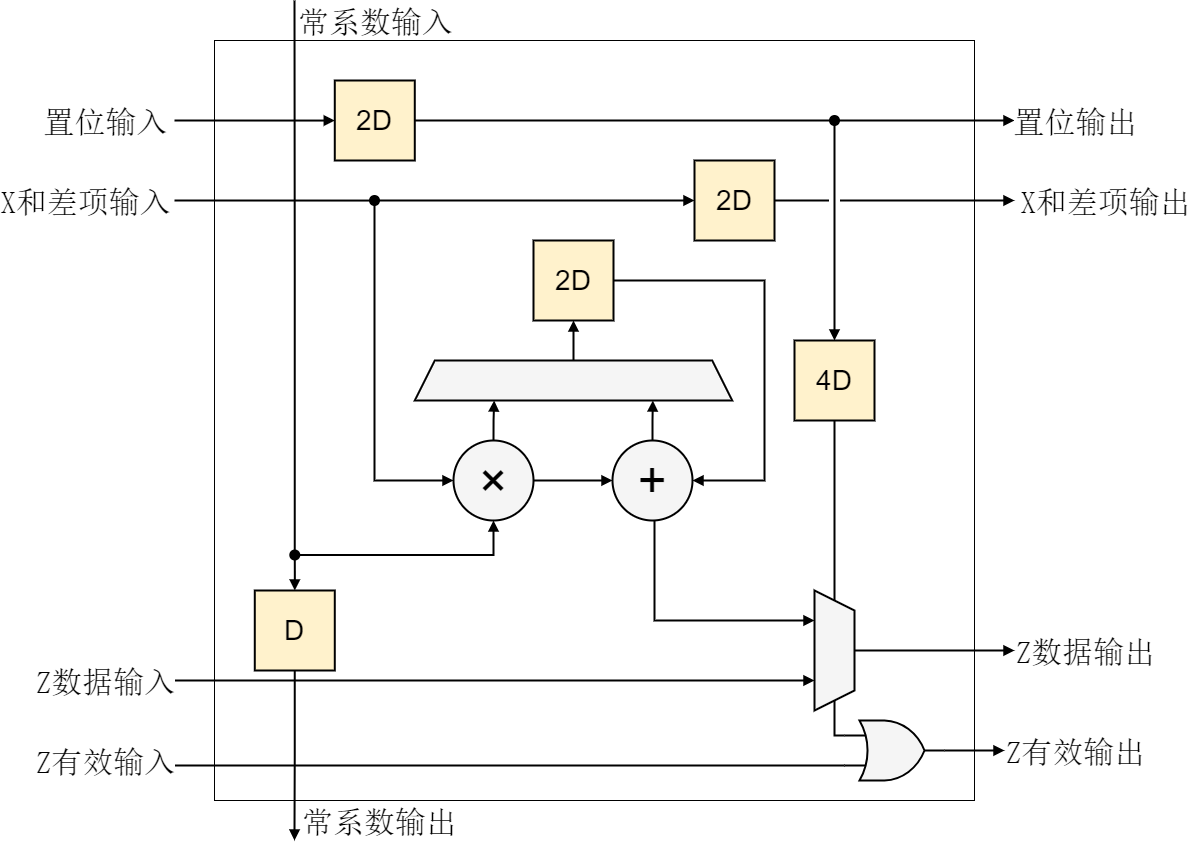
\includegraphics[scale=0.25]{./pictures/x2zPE.png}
          \caption{$Z=CX$的PE}
          \label{x2zPE}
        \end{figure}
        \begin{figure}[H]
          \centering
          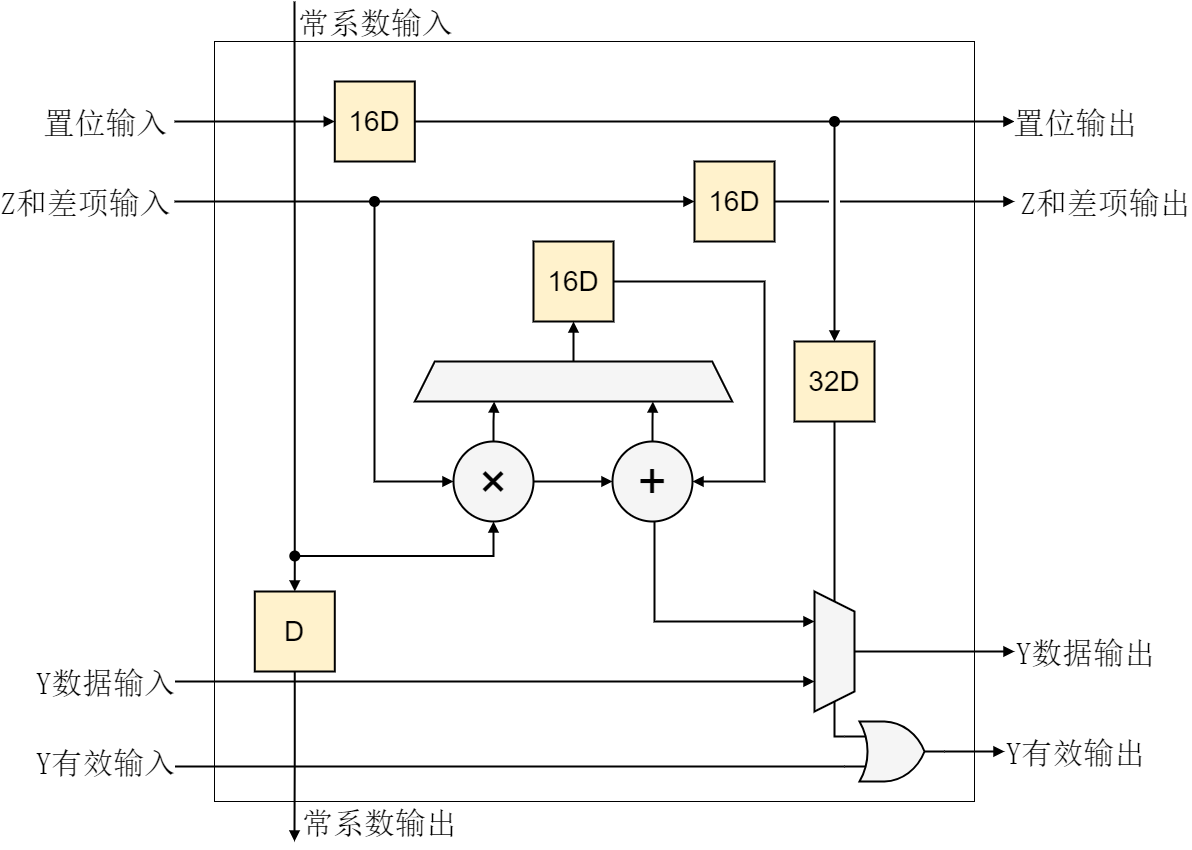
\includegraphics[scale=0.25]{./pictures/z2yPE.png}
          \caption{$Y^{T}=CZ^{T}$的PE}
          \label{z2yPE}
        \end{figure}

        以$Z=CX$中列向量元素构成的和差项$x_{00}+x_{07},x_{00}-x_{07}$到
        $x_{03}-x_{04},x_{03}+x_{04}$得到$z_{01},z_{02}$的过程为例,描述单个PE的
        运行原理。当$x_{00}+x_{07},x_{00}-x_{07}$输入时,置位输入有效。将其与余弦常
        数项输入相乘得到乘积项,再将其送进延迟2拍的移位寄存器进行暂存。当后续输入
        $x_{01}+x_{06},x_{01}-x_{06}$到$x_{03}+x_{04},x_{03}-x_{04}$输入时。置位输入无效
        移位寄存器输入为乘积和延迟2拍的输出进行累加。当$x_{03}+x_{04},x_{03}-x_{04}$
        累加后得到$z_{00},z{01}$。从$x_{00}+x_{07}$到$z_{00}$的生成经过6个时钟周期,
        因此将置位信号延迟6拍得到$z$数据输出MUX的选择信号。具体的运行时序如图
        \ref{PE运行时序}所示。
        \begin{figure}[H]
          \centering
          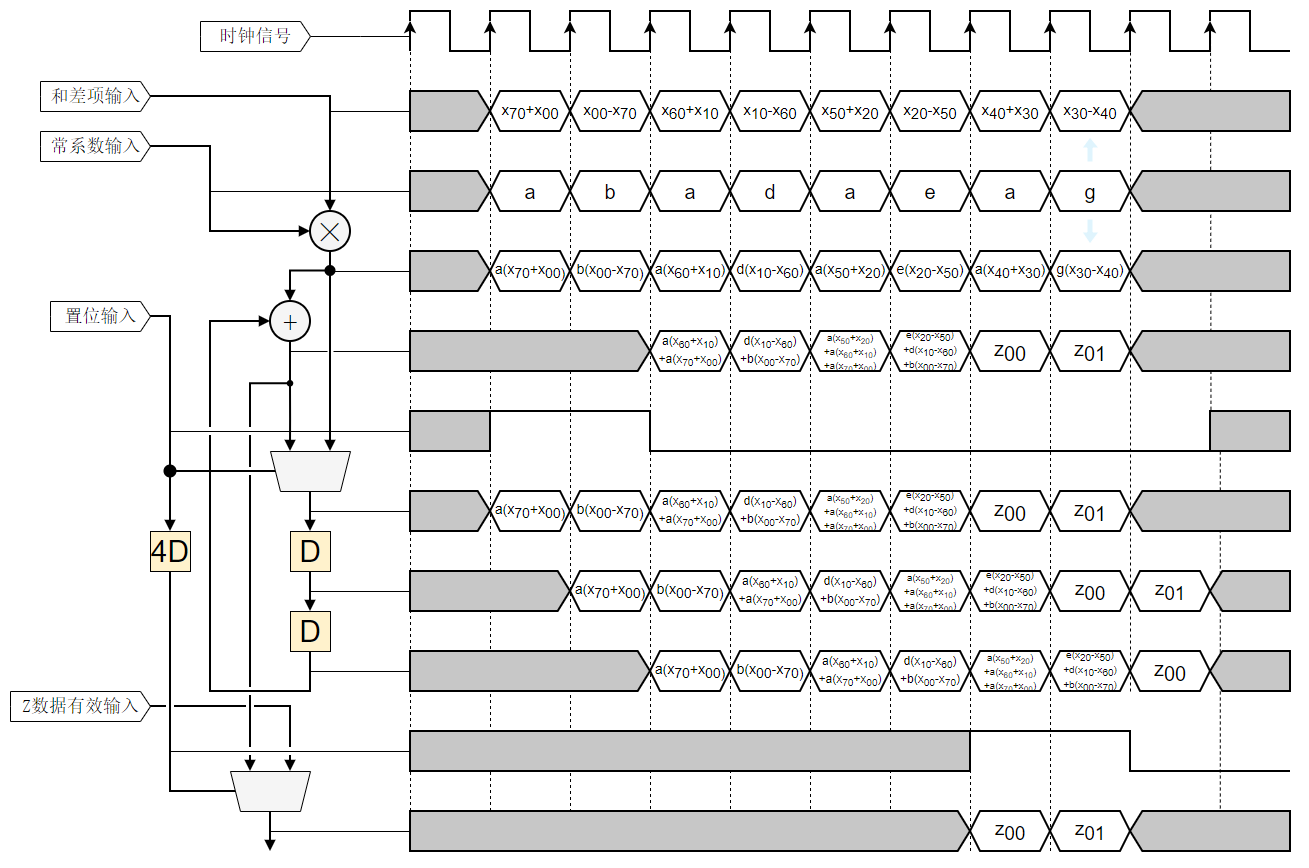
\includegraphics[scale=0.5]{./pictures/PE时序.png}
          \caption{$Z=CX$阵列PE运行时序}
          \label{PE运行时序}
        \end{figure}
        除第一列以外,每个PE的输入来自水平相邻PE的输出。除了第一行的颜色通道之外,
        每个PE的常系数输入来自垂直相邻PE的输出。第一行的常系数来自ROM。第n列的PE
        运算$z_{0,2(n-1)},z_{0,2(n-1)+1}$。为了输出$z_{00}$到$z_{07}$的串行流。如图\ref{x2zPE}
        所示,水平方向x数据延迟2拍,使运算结果z在时间上不重叠。再通过每个PE中z数据级联
        MUX和有效信号级联或门的方式使最后一列PE的Z数据输出$z_{00}$到$z_{07}$的串行流对应
        时序如图\ref{z输出时序}所示。
        \begin{figure}[H]
          \centering
          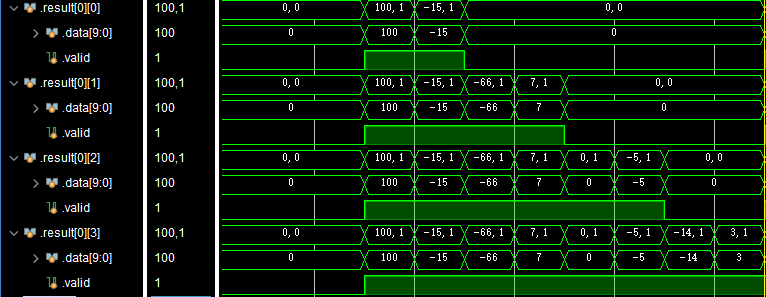
\includegraphics[scale=0.8]{./pictures/z输出时序.png}
          \caption{z输出时序}
          \label{z输出时序}
        \end{figure}
        
        通过上述过程可以得到$Z$,还需要再计算$Y^{T}=CZ^{T}$,$Z=CX$阵列依次输出
        $Z$的列向量$Z_{0},Z_{7},Z_{1},Z_{6},Z_{2},Z_{5},Z_{3},Z_{4}$
        所以需要通过$Z_{n},Z_{7-n}$输入到和差项生成模块得到$Z^{T}$列向量的和差项,
        下面通过此过程描述和差项的运行原理。
        \begin{figure}[H]
          \centering
          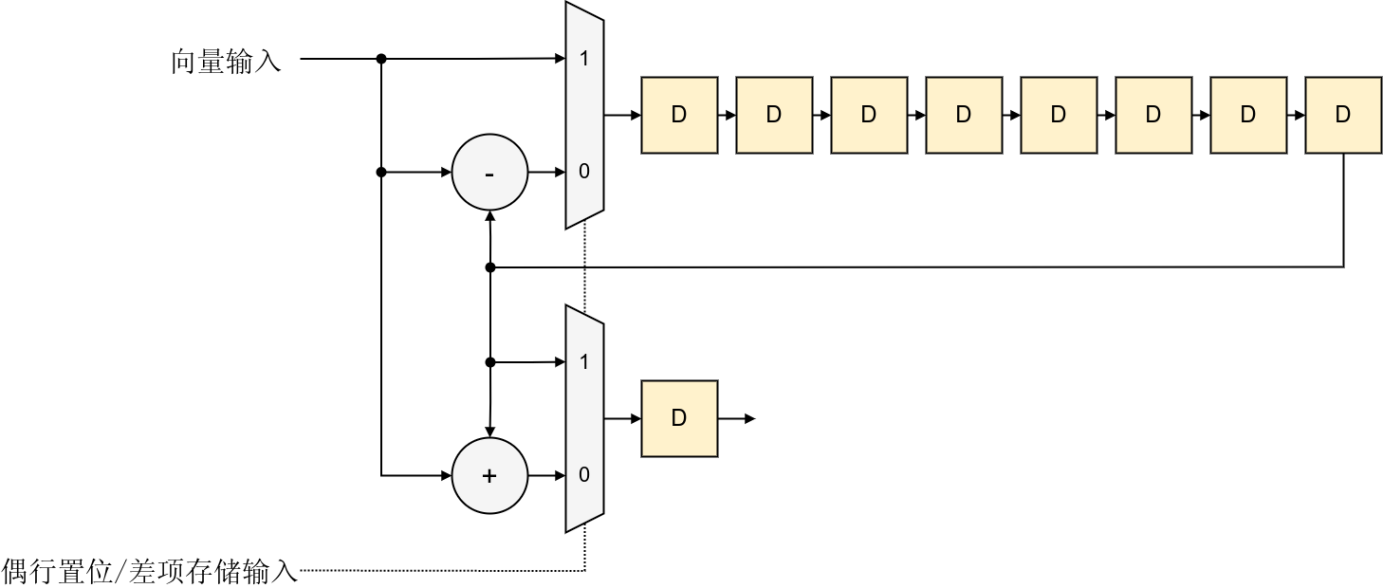
\includegraphics[scale=0.8]{./pictures/和差项生成.png}
          \caption{$Y^{T}=CZ^{T}$和差项生成模块}
          \label{和差项生成}
        \end{figure}
        \begin{figure}[H]
          \centering
          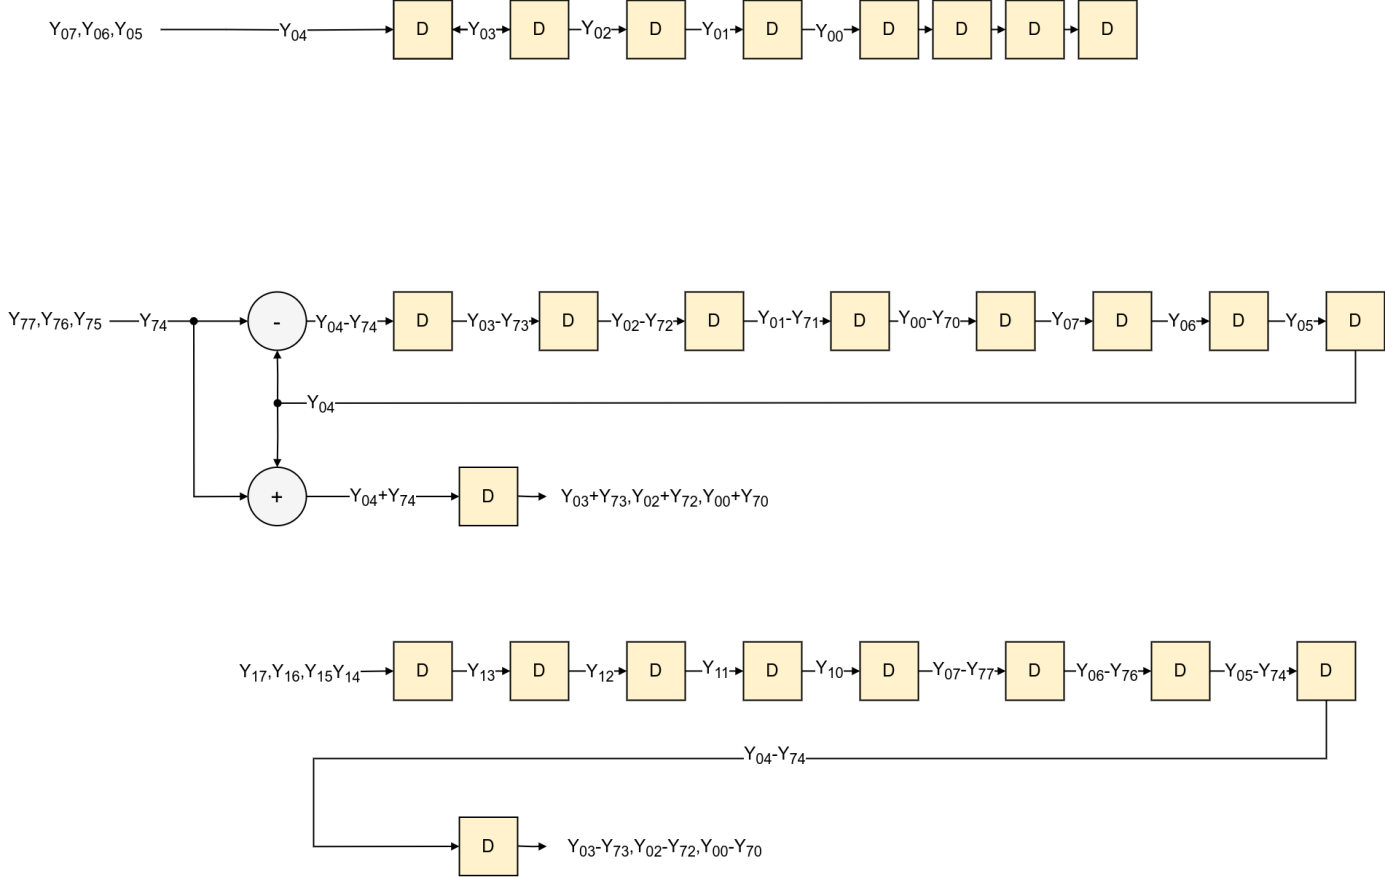
\includegraphics[scale=0.8]{./pictures/和差项生成步骤.png}
          \caption{$Z^{T}$和差项生成步骤}
          \label{和差项生成步骤}
        \end{figure}

        该结构的运行步骤如图所示,当的第1行($Z_{00}$到$Z_{07}$)输入时,偶
        行置位为1。将该行输入到8拍的移位寄存器上;当的第8行($Z_{70}$到$Z_{
        77}$)输入时,偶行置位为0。将移位寄存器输出的1行和8行输入到减法器并
        送回到移位寄存器,同时输入到加法器输出和项;当Y的第2行($Z_{10}$到$
        Z_{17}$)输入时,偶行置位为1将该行输入到8拍的移位寄存器上,同时移位
        寄存器输出上一步骤计算的差项。其他行之间的和差项运算同理。
    \subsection{Zigzag扫描模块}
      \vspace{1em}
      由于DCT模块输出的$y_{ij}$的顺序为从左到右,从上到下。所以要进行zigzag排序,
      需要把数据先写入到RAM进行暂存,经过一段延时实际后,再使用zigzag模块进行
      读出。为了最大限度提高数据的实时性,使用python脚本对写入和读出进行建模仿真
      。计算出写入和读出的延时时间最少为27个时钟周期。

      Zigzag扫描模块的内部结构划分如图\ref{zigzag module}所示。当输入数据有效时,
      计数器开启计数,计数值作为RAM的写地址。地址高低3位分别为y,x坐标。由此实现
      水平扫描写入。当计数值大于等于延迟时间时,启动zigzag扫描器读出数据。
      \begin{figure}[H]
        \centering
        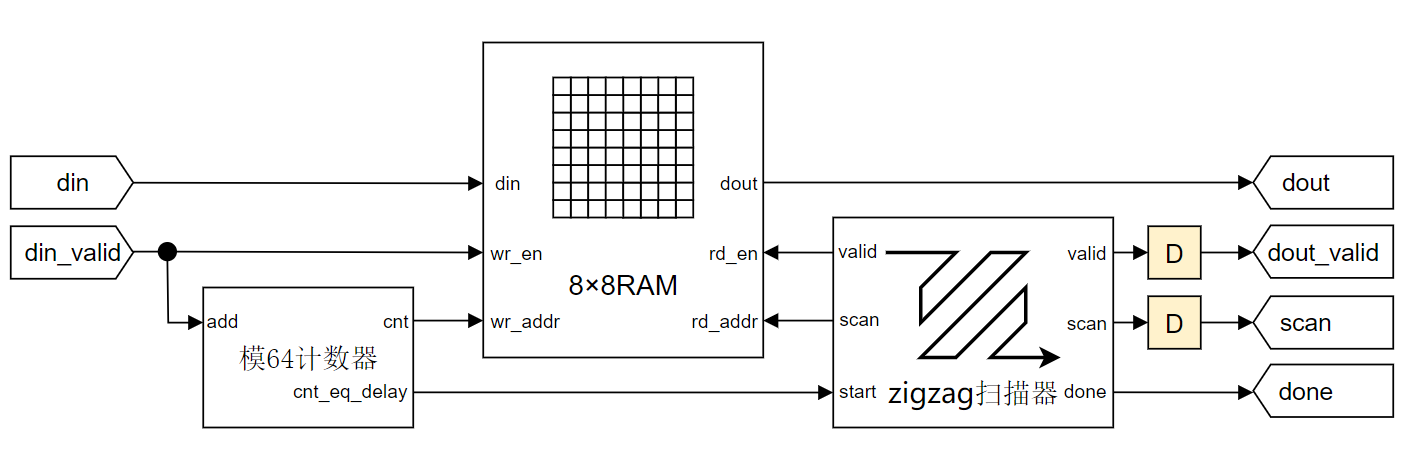
\includegraphics[scale=0.4]{./pictures/zigzagModule.png}
        \caption{Zigzag扫描模块内部划分}
        \label{zigzag module}
      \end{figure}
      
      \subsubsection{zigzao扫描器}
        \vspace{1em}
        由图\ref{scanner}所示。该模块使用一个状态来控制两个代表坐标值的计数器
        当状态机right、left信号有效时,计数器分别加一和减一。down、up信号同理。当zero
        信号有效时两个计数器清零。
        \begin{figure}[H]
          \centering
          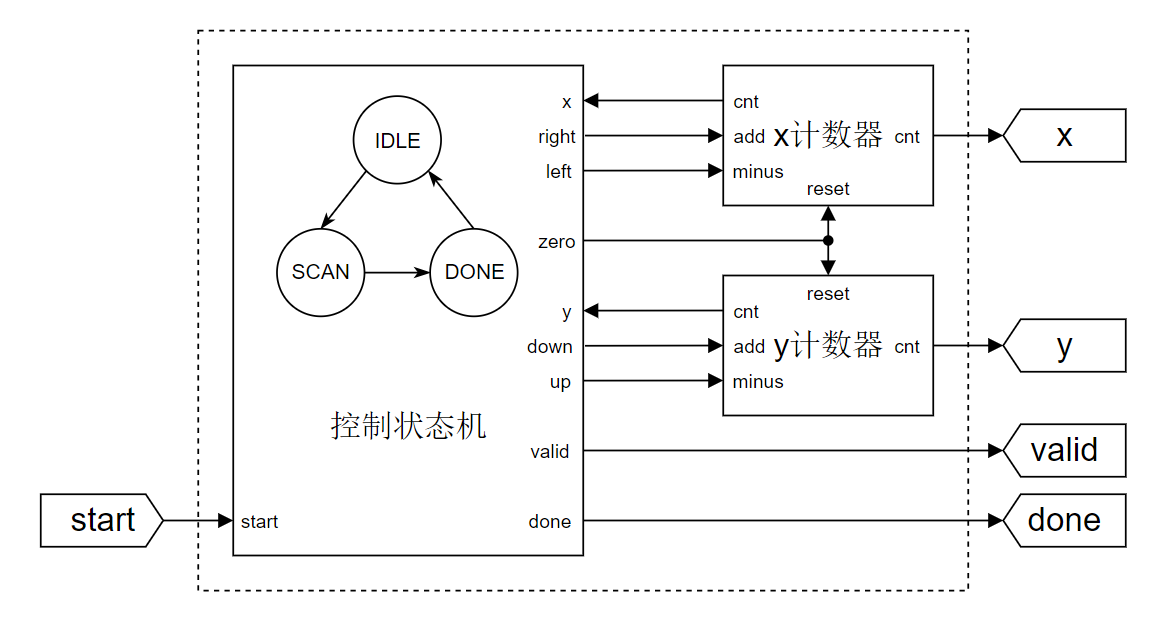
\includegraphics[scale=0.4]{./pictures/scanner.png}
          \caption{Zigzag 扫描器}
          \label{scanner}
        \end{figure}

        \begin{table}[H]
          \caption{Zigzag模块输入输出信号}
          \label{zigzag io}
          \centering
          \begin{tabular}{ccc}
            \toprule
            信号名称 & 方向 & 功能\\
            \midrule
            start & 输入 & 当高电平时启动zigzag扫描\\
            x & 输出 & zigzag扫描的水平坐标\\
            y & 输出 & zigzag扫描的垂直坐标\\
            valid & 输出 & 表示输出坐标值有效\\
            done & 输出 & 当高电平时表示zigzag扫描结束\\
            \bottomrule
          \end{tabular}
        \end{table}

        \begin{figure}[H]
          \centering
          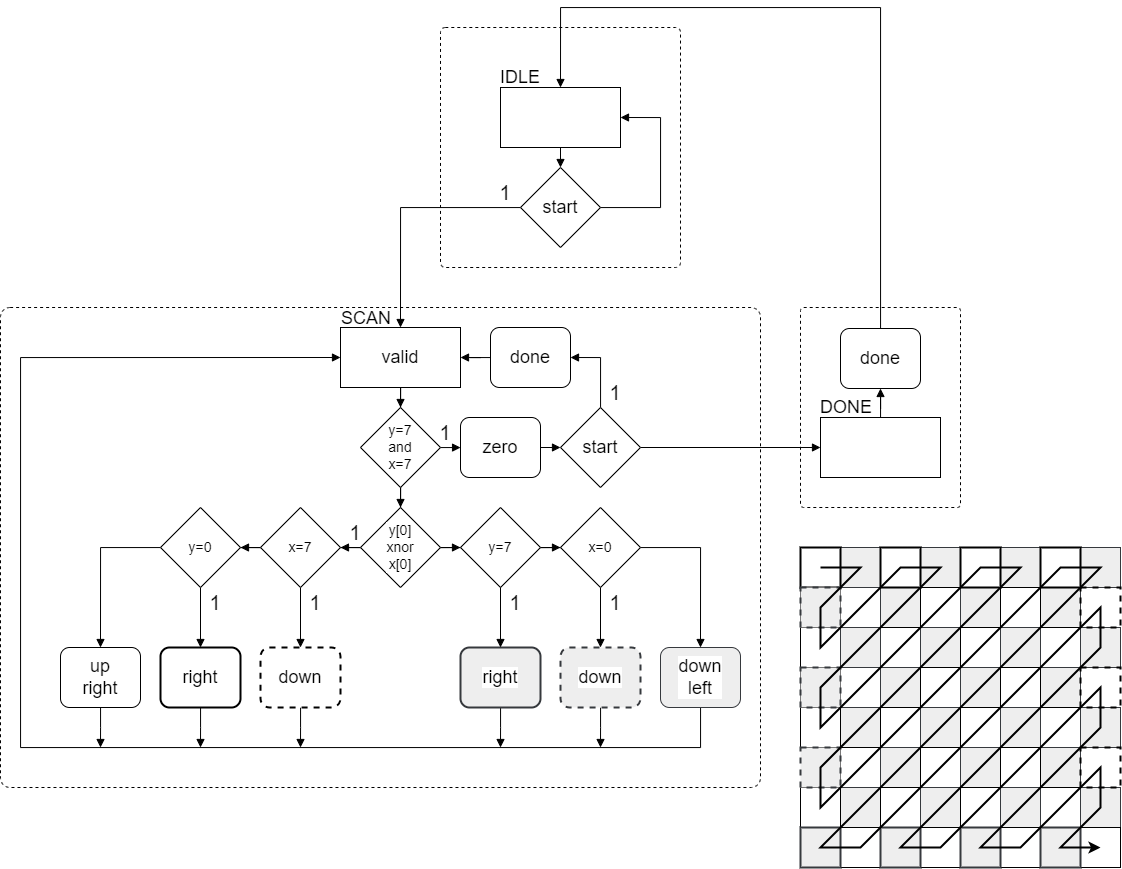
\includegraphics[scale=0.4]{./pictures/zigzag ASM.png}
          \caption{Zigzag ASM图}
          \label{zigzag ASM}
        \end{figure}

        该状态机的ASM图如图\ref{zigzag ASM}所示,在ASM图中每个虚线框代表一个状态
        每个状态中都带有一个矩形框,矩形框的左上角标注状态名称,内部存放穆尔型输出,
        同时表示该信号此时有效。与流程图类似,棱形框代表状态输入信号的判断。圆角矩
        形内部存放米利型输出。下面分别用三个状态描述zigzag扫描的运行步骤。

        初态为IDLE状态,表示该模块空闲,当接收到start信号有效时,跳转到SCAN状态开始
        工作;SCAN状态表示该模块正进行扫描,valid信号有效。如图\ref{zigzag ASM}右下角
        所示,在此状态下根据当前所在的坐标控制下个时钟的移动方向。移动的方向根据坐标分
        为6种(灰色矩形左下,灰色粗线矩形右,灰色虚线矩形下,白色矩形右上,白色粗线矩
        形右,白色虚线下矩形,)。当坐标值为$(7,7)$时,输出zero信号有效对坐标值进行清
        零,再根据start判断是否进行下一次扫描,为0时跳转到DONE状态结束扫描,为1时输
        出done信号表示本次扫描结束;DONE状态表示扫描结束输出done信号有效,并无条件
        跳转到IDLE状态。

        该模块的valid输出最终接入RAM模块的读使能。如果在清理之后直接跳转到DONE状态,会
        导致RAM的读数据有2个时钟周期的中断。如果RAM一直保持写入,就会导致RAM的吞吐
        率不一致,进而导致数据丢失。所以增加清零后SCAN状态的跳转路径。
  \subsection{量化模块}
      由于DCT模块的有些输出为组合逻辑输出,如第64个像素点。此时信号的建立时间会比较长
      ,为了不继续增加组合逻辑关键路径,就先把数据存在Zigzag扫描模块中进行缓存,再通过
      量化模块进行量化。量化最直接实现就是使用除法器进行实现。由于除法器在fpag中资源比较
      稀缺,同时工作时钟频率不高。本设计不采用除法器进行实现。考虑到量化中的除数为常数,
      同时如果被除数是2的次幂,除法运算就相当于右移运算。如式(\ref{qeuatizer equation})
      可以将除法分解为一次乘法再进行一次2次幂的除法(移位),当n越大时,精度就越大。这样
      就可以使用乘法器实现除数为常数的除法。本设计采用$2^{16}$作为其中的被除数。
      \begin{equation}
        \frac{F(u,v)}{Q(u,v)}=F(u,v)*\frac{\left(\frac{2^{n}}{Q(u,v)}\right)}{2^{n}}
        \label{qeuatizer equation}
      \end{equation}
      量化器的RTL视图如图\ref{quantizer}。将对应的乘数$\frac{2^{16}}{Q(u,v)}$存进ROM中,把
      Zigzag模块的扫描输出作为ROM的读地址输入。进而获取对应的乘数,再将乘积进行右移截
      位得到最终的量化值。
      \begin{figure}[H]
        \centering
        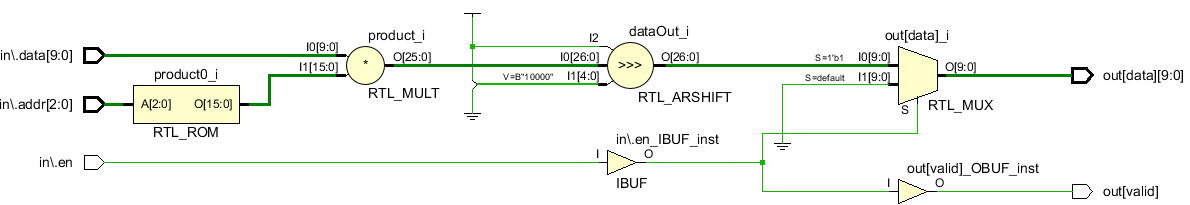
\includegraphics[scale=0.5]{./pictures/quantizer.png}
        \caption{量化器结构图}
        \label{quantizer}
      \end{figure}


  \subsection{熵编码模块}
    熵编码模块读取颜色通道量化后的数据并生成压缩码流。该模块的结构如图\ref{enropyCoder}
    所示数据依次进入中间码生成模块、EOB生成模块、Huffman编码模块以及不定长数据拼接模块。
    \begin{figure}[H]
      \centering
      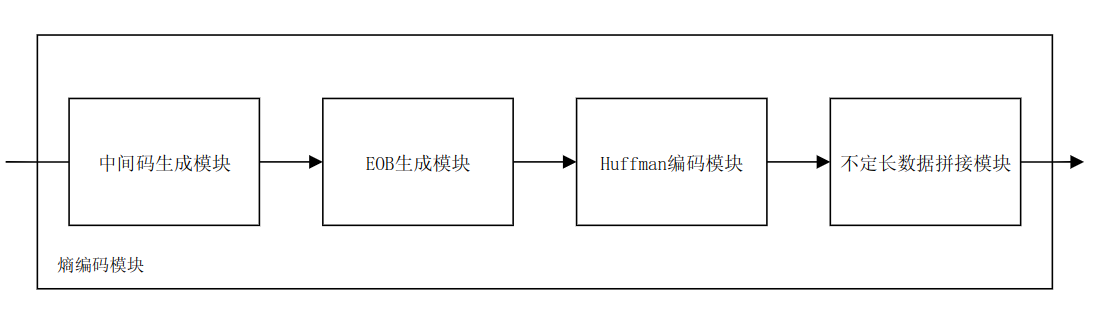
\includegraphics[scale=0.4]{./pictures/熵编码模块.png}
      \caption{熵编码模块}
      \label{enropyCoder}
    \end{figure}
    \subsubsection{中间码生成模块}
      \vspace{1em}
      如第二章所述,在进行霍夫码编码前需要将数据转换成一种中间格式,对与DC直流系数。需要
      上一个8乘8单元的差值的VLI码,即如果数值为负取其绝对值的反码,为正则取其原码。同时
      要获取数据的有效长度。对应AC交流系数,还需要改系数前0值的数量。
      \begin{figure}[H]
        \centering
        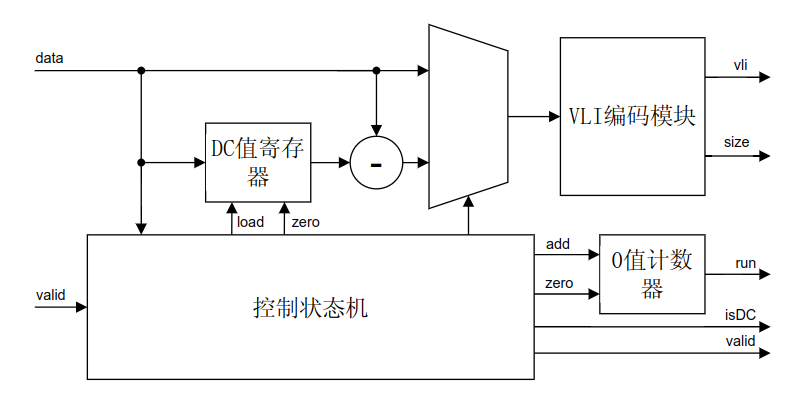
\includegraphics[scale=0.4]{./pictures/中间码生成模块.png}
        \caption{中间码模块}
        \label{tempGen}
      \end{figure}

      \begin{figure}[H]
        \centering
        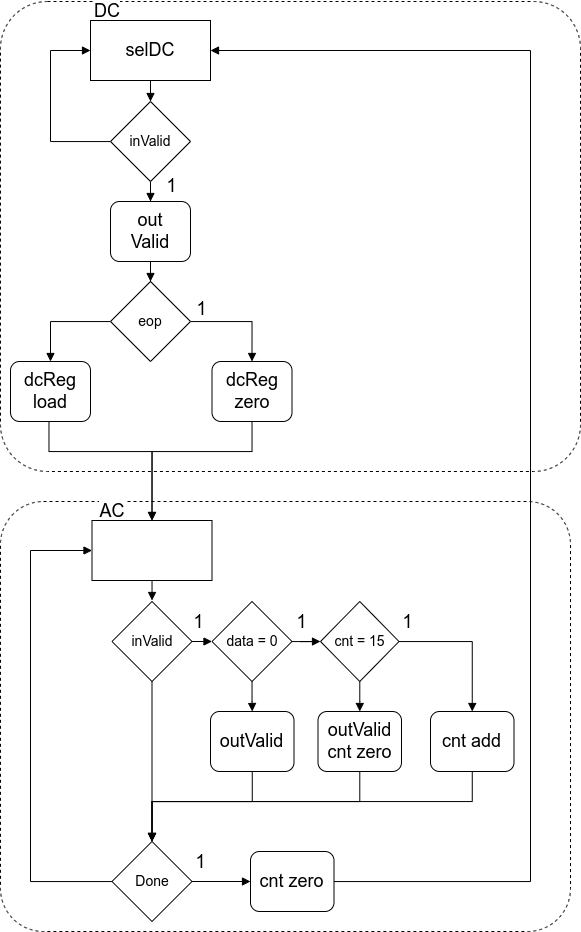
\includegraphics[scale=0.4]{./pictures/tmepCodeASm.png}
        \caption{中间码模块ASM图}
        \label{tempGenASM}
      \end{figure}

      该模块的数据通路如图\ref{tempGen},控制状态机的ASM图如图\ref{tempGenASM}所示。通过
      一个MUX选择VLI编码模块的输入是来自于DC系数和AC系数。VLI模块解析数据获取其有效长度和
      VLI码。

      在VLI编码模块中,为了获取数据的尺寸,即绝对值的有效长度。可以利用与二进制值与自身的
      补码按位相与得到低位到高位的第一个1的独热码的特点。将绝对值的高低颠倒进行此操作的到
      高位到低 位到最高有效位为1的独热码,再将其输入到编码器得到其尺寸。
      
      在未收到数据前,状态机处于DC状态 在该状态下MUX选择数据输入与DC寄存器的差值。
      当数据有效时,则为8乘8单元的第一个数据即DC值,将其值与上一个DC值作差。再将差值送入
      VLI编码模块中得到有效长度size和其VLI码,同时判断帧尾有效信号eop是否有效,如果有效
      则将DC寄存器置0,否则加载当前DC系数,供下一个8乘8单元使用,同时使能信号isDC有效,
      表示当前输出为DC系数,接着在下一个时钟周期跳转到AC状态。

      在AC状态下,当输入数据有效时,判断其是否为0。如果为0检查零值计数器是否为15,如果为15
      则时能输出有效信号,表示输出ZRL。如果不为15则使能0值计数器自増信号。如果输入数据不为
      0值,使能输出有效信号输出该值的VIL和size,再使能零值清零信号,零值计数器将在下一个时钟
      周期清零。当输入信号done有效时说明此时为8x8单元最后一个数据,跳转回DC状态同时清零值
      计数器,输出done信号有效此时输入为零时,则不输出使能。表示当前为EOB。

    \subsubsection{EOB生成模块}
      \vspace{1em}
      EOB生成模块需要将EOB前的ZRL进行清除,以符合正确的编码规则,否则将导致数据解码失败。
      图\ref{EOBGen}为EOB生成模块,由图可知输出数据来自模块输入或FIFO。其中FIFO的输入来自模
      块输入。FIFO的写入写出以及模块输出的选择由一个状态机进行控制,图\ref{EOBGenASM}为其ASM图。

      \begin{figure}[H]
        \centering
        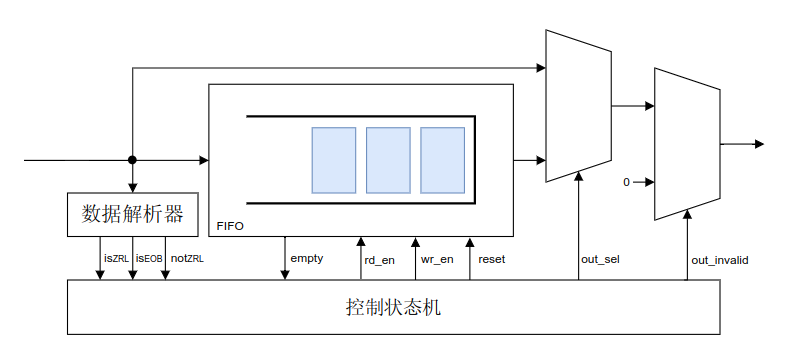
\includegraphics[scale=0.6]{./pictures/EOB生成模块.png}
        \caption{EOB生成模块}
        \label{EOBGen}
      \end{figure}

      状态机接收数据解析器的三个输出以及FIFO的空信号,当数据有效时,数据解析器对应的信号便会
      使能。数据解器的三个输出isZRL,isEOB,NotZRL。分别表示此时输入数据为ZRL,EOB,以及其余
      情况。

      状态机的初态为NORMAL状态,在该状态下如果数据为ZRL则会写入到FIFO中同时控制outInvalid时
      输出数据无效。当数据为EOB时则会FIFO进行复位清除掉之前存入的ZRL。当输入为不为ZRL和EOB时
      将检查FIFO是否为空,若为空则输出该数据。否则应先输出FIFO中的ZRL,进而跳转到RD\_FIFO状态
      同时将当前输入存入FIFO。

      在FIFO\_RD状态下,将保持FIFO读出有效。当FIFO不为空时输出FIFO的输出,当输入数据有效时将 
      会存进FIFO。当FIFO为空时,则输出则选择来自模块输入的数据同时在下一个时钟周期跳转回NORMAL
      状态。

      \begin{figure}[H]
        \centering
        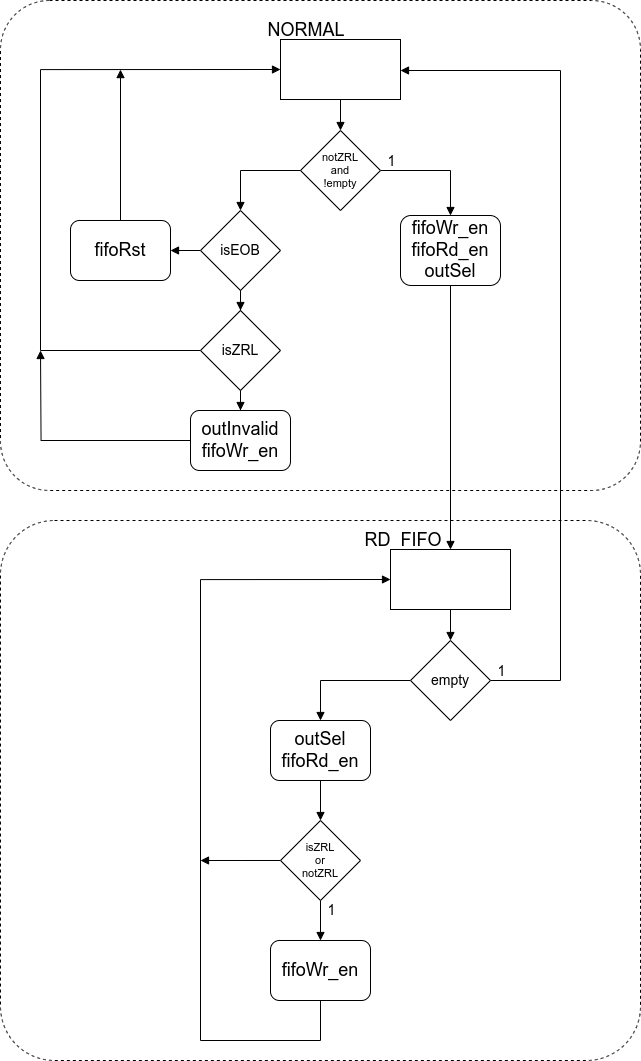
\includegraphics[scale=0.4]{./pictures/EOBGenASM.png}
        \caption{EOB生成模块ASM图}
        \label{EOBGenASM}
      \end{figure}

    \subsubsection{Huffman编码模块}
      \begin{figure}[H]
        \centering
        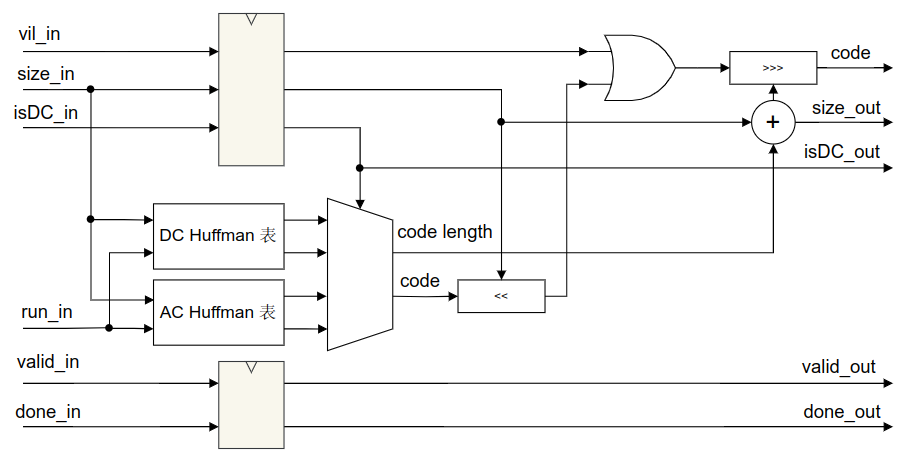
\includegraphics[scale=0.4]{./pictures/HuffmanCoder.png}
        \caption{Huffman编码模块}
        \label{HuffmanCoder}
      \end{figure}

      Huffman编码模块如图\ref{HuffmanCoder},该模块将输入VLI码的有效大小size和游程值作为DC、AC
      Huffman表的输入得到其Huffman码值code和码长size。再通isDC信号选择其对应的Huffman表。由于
      Huffman表采用ROM存储同时为了保证关键路径,输出会晚一个时钟周期,所以需要对其他信号也进行一次
      打拍延时以对齐时序。接着使用桶形移位寄存器将Huffman编码的按照VLI码的有效长度进行左移,再
      与VLI码进行按位相或进行拼接。由于JPEG编码是按照高位往低位的方式进行解码。因此将huffman码长
      和VLI码长相加,再使用该值对先前拼接后的编码对齐进行环形右移。将编码进行高位对齐最后将该值
      和总长度输出,得到变长编码。
     
    \subsubsection{不定长数据拼接模块}
    \vspace{1em}
      Huffman编码模块的输出数据是由编码和码长构成的不定长不数据。在最终输出的压缩码流中是没有对应
      的码长数据的。各个数据是通过解高位的Huffman编码获取对应的码长和中间的零值,因此需要将对应每个
      8乘8单元每个部分对应的编码进行从高位到低位的拼接。因此需要一个该模块对变长码进行拼接得到定
      长码。

      该模块输出宽度为64位的定长编码。考虑到之后的JPEG数据生成模块需要接收三个颜色通道,并且整合到
      一个输出,为了提高其吞吐量,该模块对输入数据进行了依次串并转换。对数据进行了一定地缓存,防止
      了后级模块的吞吐量不足导致的数据丢失。
      \begin{figure}[H]
        \centering
        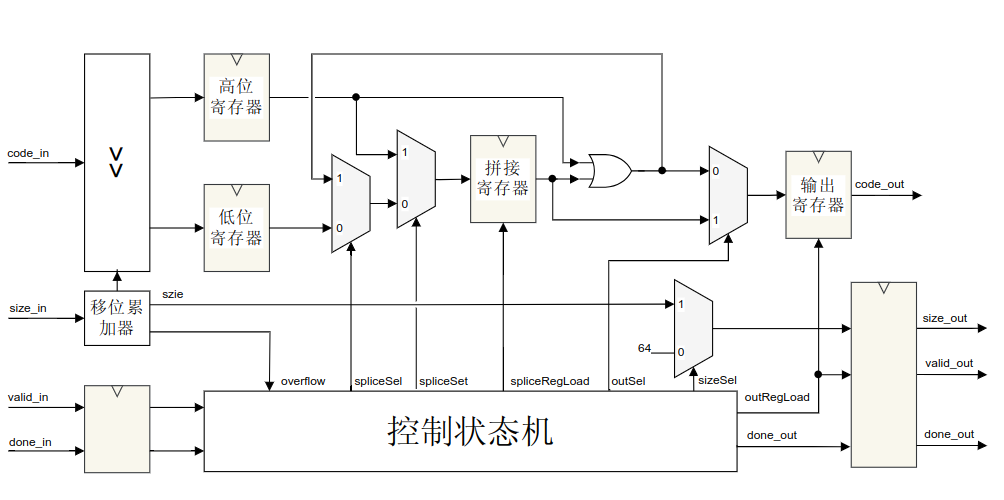
\includegraphics[scale=0.4]{./pictures/拼接模块.png}
        \caption{不定长数据拼接模块}
        \label{spliceModule}
      \end{figure}

      图\ref{spliceModule}为该模块的数据通路。该模块向使用桶形移位寄存器来对数据进行移位,使用一个
      累加器定位当前输入编码的移位值。其桶形移位器的输入为64×2=128位。高64为连接输入数据,低64位补
      0。移位后的高64位和低64位分别存入高位寄存器和低位寄存器。使用一个拼接寄存器存储目前所拼接
      的编码。以及一个输出寄存器占存上次输出的64位定长码。由一个控制状态机来操作这些寄存器的加载和
      数据的输出。

      \begin{figure}[H]
        \centering
        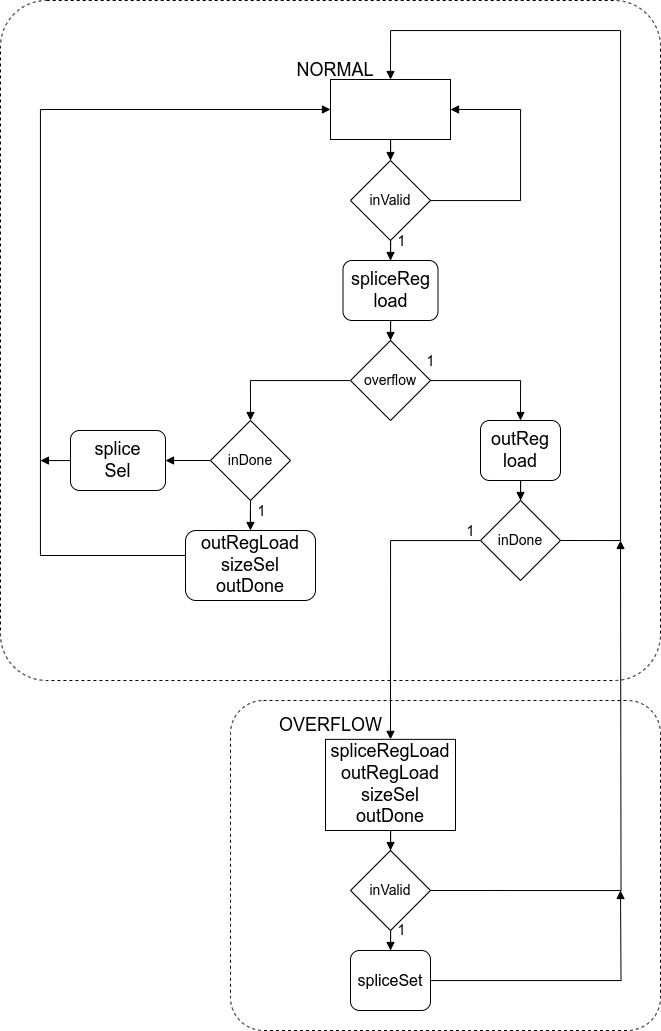
\includegraphics[scale=0.5]{./pictures/spliceASM.png}
        \caption{不定长数据拼接模块ASM图}
        \label{spliceASM}
      \end{figure}
      
      当输入数据有效时,移位器根据当前的移位累加值,对其进行右移。如果当将的累加值加输入数据的累加值小
      于64。累加器会在下一个时钟周期更新与当前码长的累加值。当输入码长加累加值大于等于64时,移位后高
      位寄存器以满64位,会溢出一部分数据到低位寄存器(大于64时),这时累加器在下一个时钟周期会更新溢出
      的比特数,即输入码长加累加值减64,同时输出溢出信号overflow有效。当输入端口的done信号有效时,则
      代8乘8单元的最后一个编码输入,在下一个时钟周期累加值清零,供下一个8乘8单元定位当前移位长度,同时
      更新一个寄存输出size,供后续输出未满64位编码时,编码的有效长度,当输入编码长度加累加值小于等于
      64时,更新其值。否则更新输入码长加累加值减64。

      控制状态机有两个状态NORMAL和OVERFLOW。其初态为NORMAL状态,当移位器的输出有效时,输出spliceRegLoad
      有效。拼接寄存器在下一个时钟周期将会更新,当溢出信号overflow无效同时done无效时,spliceSel使拼接寄
      存器的次态选通现态与高位寄存器按位相或,与存储在高位寄存器的输入编码进行拼接下面称该信号为拼接值。
      当溢出信号overflow无效同时done有效时,输出寄存器次态选通拼接值,拼接寄存器次态选通低位寄存器。由于
      目前高位寄存器未溢出,所以低位寄存器为0。将其送入拼接寄存器使其清零,以供拼接后续输入数据。当overfolw
      有效时,拼接寄存器次态接通包含溢出数据的低位寄存器。outRegLoad有效输出寄存器下个时钟周期加载拼接值,
      当done有效时需要在输出拼接值后再输出溢出值,将状态跳转到OVERFLOW。

      在OVERFLOW状态下,模块输出此时输出满64位的拼接值,下一个时钟周期输出寄存器需要加载位于拼接寄存器
      的溢出值,因此使能outRegLoad和outSel。同时输出OutDone和size有效表示8乘以8单元最后一个数据和有效长度。
      在该状态下拼接寄存器也需要使能spliceRegLoad进行加载,如果此时移位器输出有效,使能spliceSet加载高位寄
      存器。否则则加载低位寄存器进行清零。

  \subsection{JPEG数据生成模块}
    \vspace{1em}
    jpeg数据生成模块负责将3个颜色通道整合到一个输出端口进行输出,本设计采用采样格式为YCbCr444,所以一个MUC
    中包含三个颜色通道各一个8乘8单元。

    \begin{figure}[H]
      \centering
      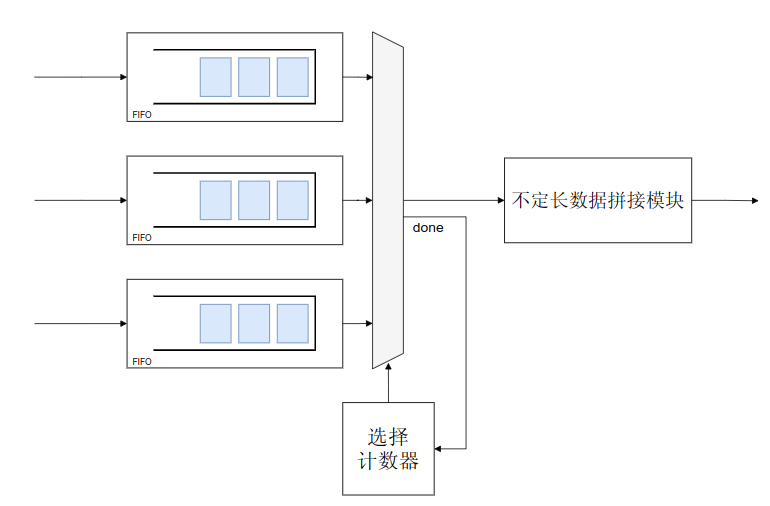
\includegraphics[scale=0.4]{./pictures/数据生成模块.png}
      \caption{JPEG数据生成模块}
      \label{数据生成模块}
    \end{figure}

    图\ref{数据生成模块}为该模块的大致结构。每个颜色通道都是用一个FIFO进行缓存,当对应的颜色通道不被后级模块
    读取时能够即使缓存,以免数据丢失。当选中的fifo输出读到对应的done信号有效时则,将选择计数器加一切换到另一
    代表该通道的8乘8单元读取完毕,切换到下个颜色通道,进行轮转读取进而拼接。当Cr通道的FIFO读取到eop和done信号同时有效
    时代表读取了完整的一帧数据,使能不定长数据的done信号。

  \subsection{本章总结}
    \vspace{1em}
    本章系统地阐述了JPEG编码系统的硬件架构设计与实现方法。在整体设计思路上,通引入流水线技术将复杂的编码流程分解
    为多级处理单元。显著提升了数据的吞吐量力;在DCT的实现上采用了二维脉动阵列优化了计数效率。器规则化的处理单元
    保持了较高的运算并行度;针对数据缓存需求设计的乒乓操作机制。有效地解决了跨时域传输中的速率匹配问题。熵编码模块
    构建了完整压缩数据生成流水线。其模块化的设计思路和优化方法也为其他实时图像处理系统的开发提供了有价值的参考。
  

\newpage
\section{JPEG编码系统仿真结果与指标分析}
  \vspace{1em}
  \subsubsection{编码模块仿真}
  \begin{figure}[H]
    \centering
    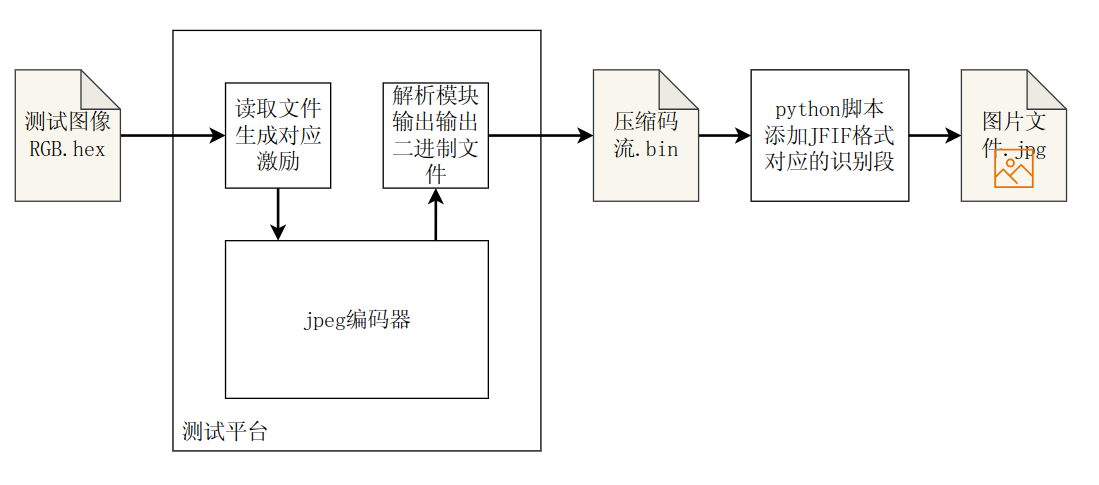
\includegraphics[scale=0.4]{./pictures/test_ele.png}
    \caption{测试环境}
    \label{test}
  \end{figure}
  本设计使用systemverilog进行RTL级描述和测试。在EDA软件vivado进行综合和仿真。编码模块的测试环境如图\ref{test}。
  验证平台读取有含有图像rgb数据的16进制的字符文件,并将其转换为符合编码模块输入的信号激励。同时读取并解析模块
  输出的压缩码流,并将其内容写入到二进制文件中。在使用python脚本添加符合JFIF格式的识别段最终输出jpg格式的文件
  使用的图片查看器进行查看。

  \begin{figure}[H]
    \centering
    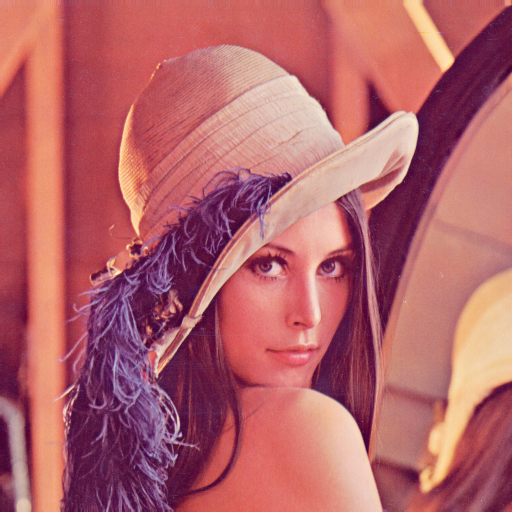
\includegraphics[scale=0.4]{../src/test/test_img512x512.png}
    \caption{测试原图像}
    \label{origin image}
  \end{figure}

  作为测试输入的原图像如图\ref{origin image}所示。

  \begin{figure}[H]
    \centering
    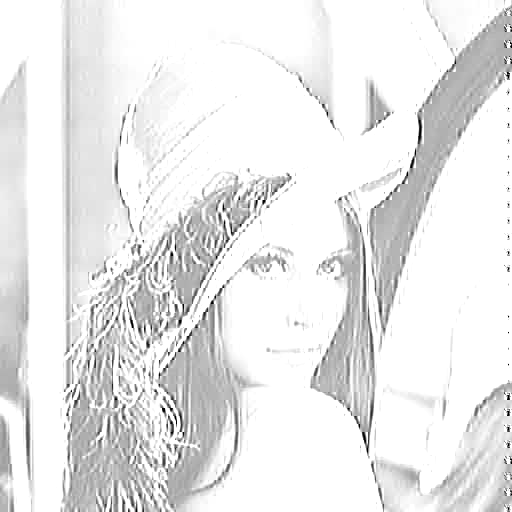
\includegraphics[scale=0.4]{../src/test/Y_channal.jpg}
    \caption{编码后的图像Y通道}
    \label{Y channal image}
  \end{figure}
  \begin{figure}[H]
    \centering
    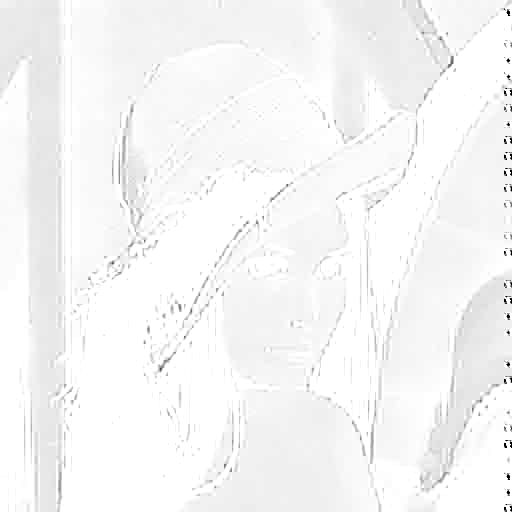
\includegraphics[scale=0.4]{../src/test/Cb_channal.jpg}
    \caption{编码后的图像Cb通道}
    \label{Cb channal image}
  \end{figure}
  \begin{figure}[H]
    \centering
    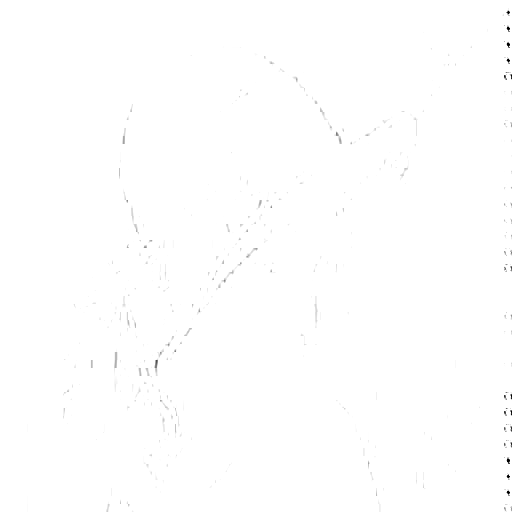
\includegraphics[scale=0.4]{../src/test/Cr_channal.jpg}
    \caption{编码后的图像Cr通道}
    \label{Cr channal image}
  \end{figure}
  \begin{figure}[H]
    \centering
    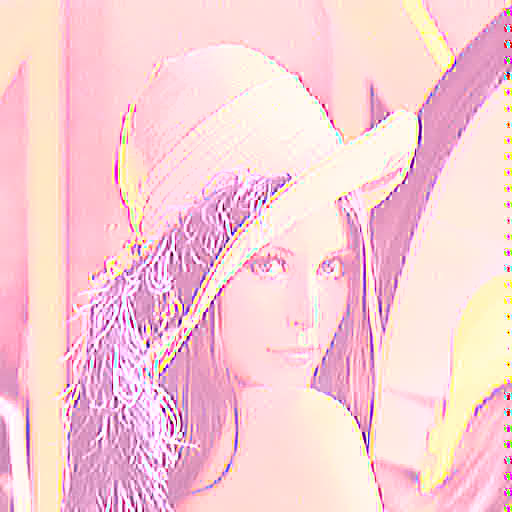
\includegraphics[scale=0.4]{../src/test/decode.jpg}
    \caption{解码后的图像}
    \label{decode image}
  \end{figure}

  最终模块输出并解码的三个颜色通道的图片如图\ref{Y channal image},\ref{Cb channal image},\ref{Cr channal image}
  所示。最终解码后的图片如图\ref{decode image}表统计了压缩前后的各项参数指标。

  \begin{table}[H]
    \caption{压缩图像的各个属性指标}
    \label{image vs}
    \centering
    \begin{tabular}{ccccc}
      \toprule
      图片名称 & 分辨率 & 文件大小(bytes) & 压缩比 & 每像素比特数\\
      \midrule
      原图像 & 512*512 & 786,432 & 1 & 24\\
      Y通道压缩图像 & 512*512 & 18,432 & 42 & 0.571\\
      Cb通道压缩图像 & 512*512 & 6,656 & 118 & 0.203\\
      Cb通道压缩图像 & 512*512 & 6,758 & 116 & 0.206\\
      压缩后的图像 & 512*512 & 31,846 & 25 & 0.96\\
      \bottomrule
    \end{tabular}
  \end{table}
  \begin{figure}[H]
    \centering
    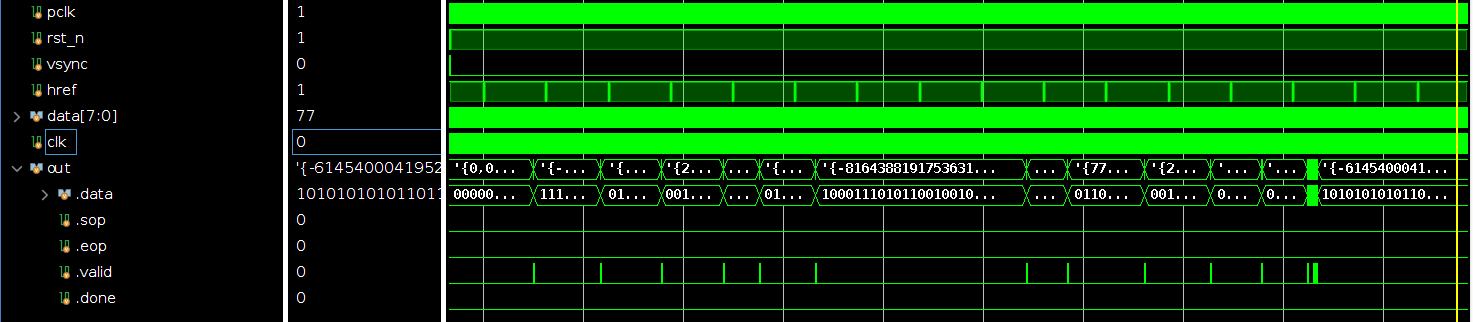
\includegraphics[scale=0.30]{./pictures/top_wave.png}
    \caption{编码模块仿真波形}
    \label{top_wave}
  \end{figure}
  编码模块仿真波形如图\ref{top_wave}所示
  \subsection{数据解析模块功能仿真}
    \vspace{1em}
    \subsubsection{读写状态机功能仿真}
      \vspace{1em}
      \begin{figure}[H]
        \centering
        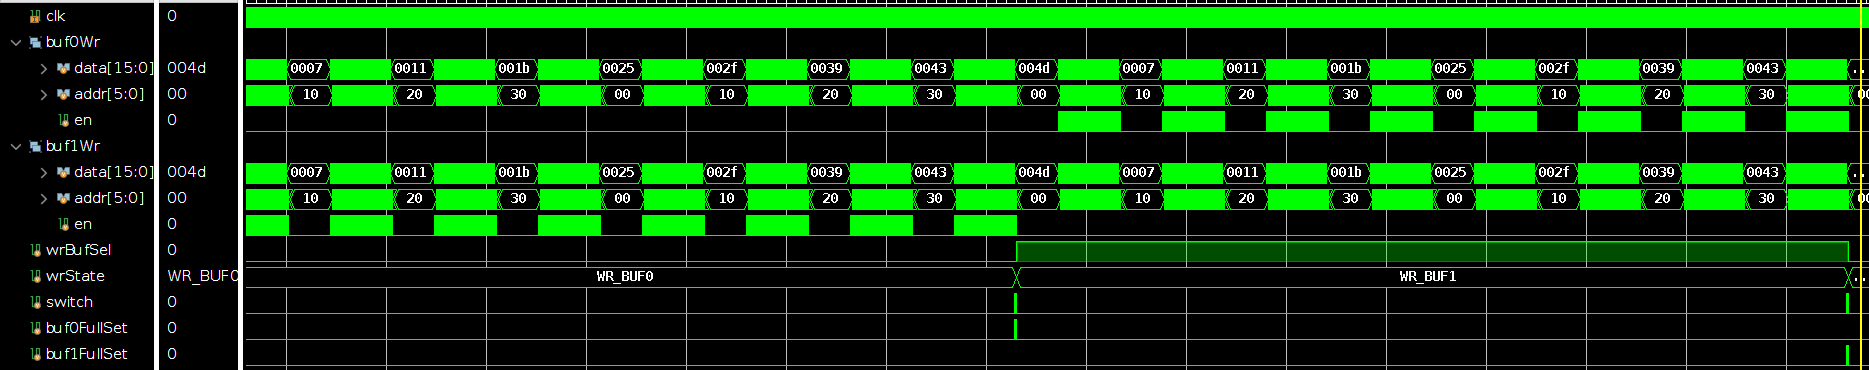
\includegraphics[scale=0.25]{./pictures/wrFSMSim.png}
        \caption{写状态机仿真波形}
        \label{WRFSMSimWave}
      \end{figure}
      写状态机的仿真波形如图\ref{WRFSMSimWave}所示,可以看出在WR\_BUF0
      状态下对BUF0的写使能信号有效,对BUF0进行写入。switch信号有效后切
      换到WR\_BUF1状态,同时输出窄脉冲信号buf0FullSet。BUF1跳转到BUF0
      同理。
      
      \begin{figure}[H]
        \centering
        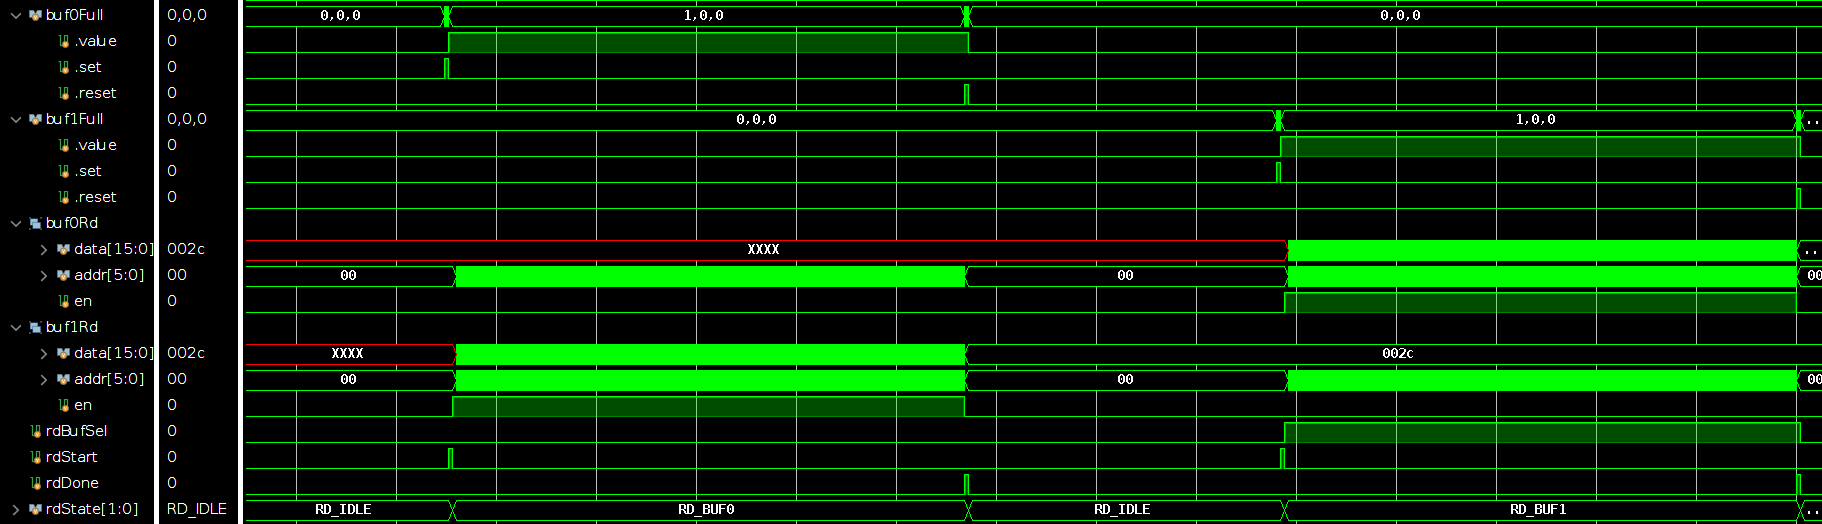
\includegraphics[scale=0.25]{./pictures/rdFSMSim.png}
        \caption{读状态机仿真波形}
        \label{RdFSMSimWave}
      \end{figure}
      读状态机的仿真波形如图\ref{WRFSMSimWave}所示,可以看到在RD\_IDLE模式
      下BUF0的满信号有效时,跳转到RD\_BUF0状态并输出start信号有效,对BUF0
      进行读取。单读取完毕输出done信号有效是回到RD\_IDLE状态并将BUF0的满信
      号置0。等待buf1写完毕满信号置1跳转到RD\_BUF1状态,在RD\_BUF1状态下与
      RD\_BUF0状态同理。
  \subsection{DCT模块功能仿真}
    \vspace{1em}
    DCT 模块中运算DCT的模块RTL视图如图\ref{DCTSchematice}所示。其中in[0],
    out[0]、in[1],out[1]、in[2],out[2]表示三个颜色通道的输出输出。
    \begin{figure}[H]
      \centering
      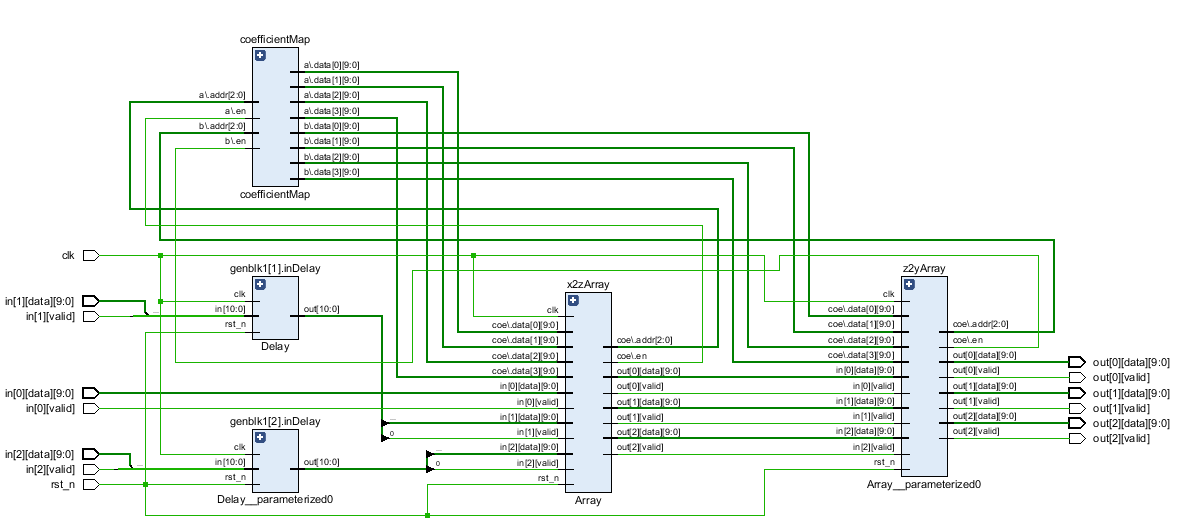
\includegraphics[scale=0.5]{./pictures/DCTSchematice.png}
      \caption{DCT运算部分RTL视图}
      \label{DCTSchematice}
    \end{figure}
    下面以一个8×8单元输入为激励进行仿真,仿真后的波形如图\ref{DCTSimulationWave}
    其中灰色波形为Y通道,绿色波形为Cr通道,蓝色波形为Cb通道。由图可知从X到Z的
    时滞为7个时钟周期,从Z到Y的时滞为56个时钟周期,所以整模块的时滞为63。由公式
    (\ref{8*8 2D-DCT})可知输出$Y(u,v)$的每个元素都需要$X(i,j)$64个元素进行计算,
    所以当数据串行输入时,理论极限最小时延为63个时钟周期,本设计时沿达到理论极限。
      \begin{figure}[H]
        \centering
        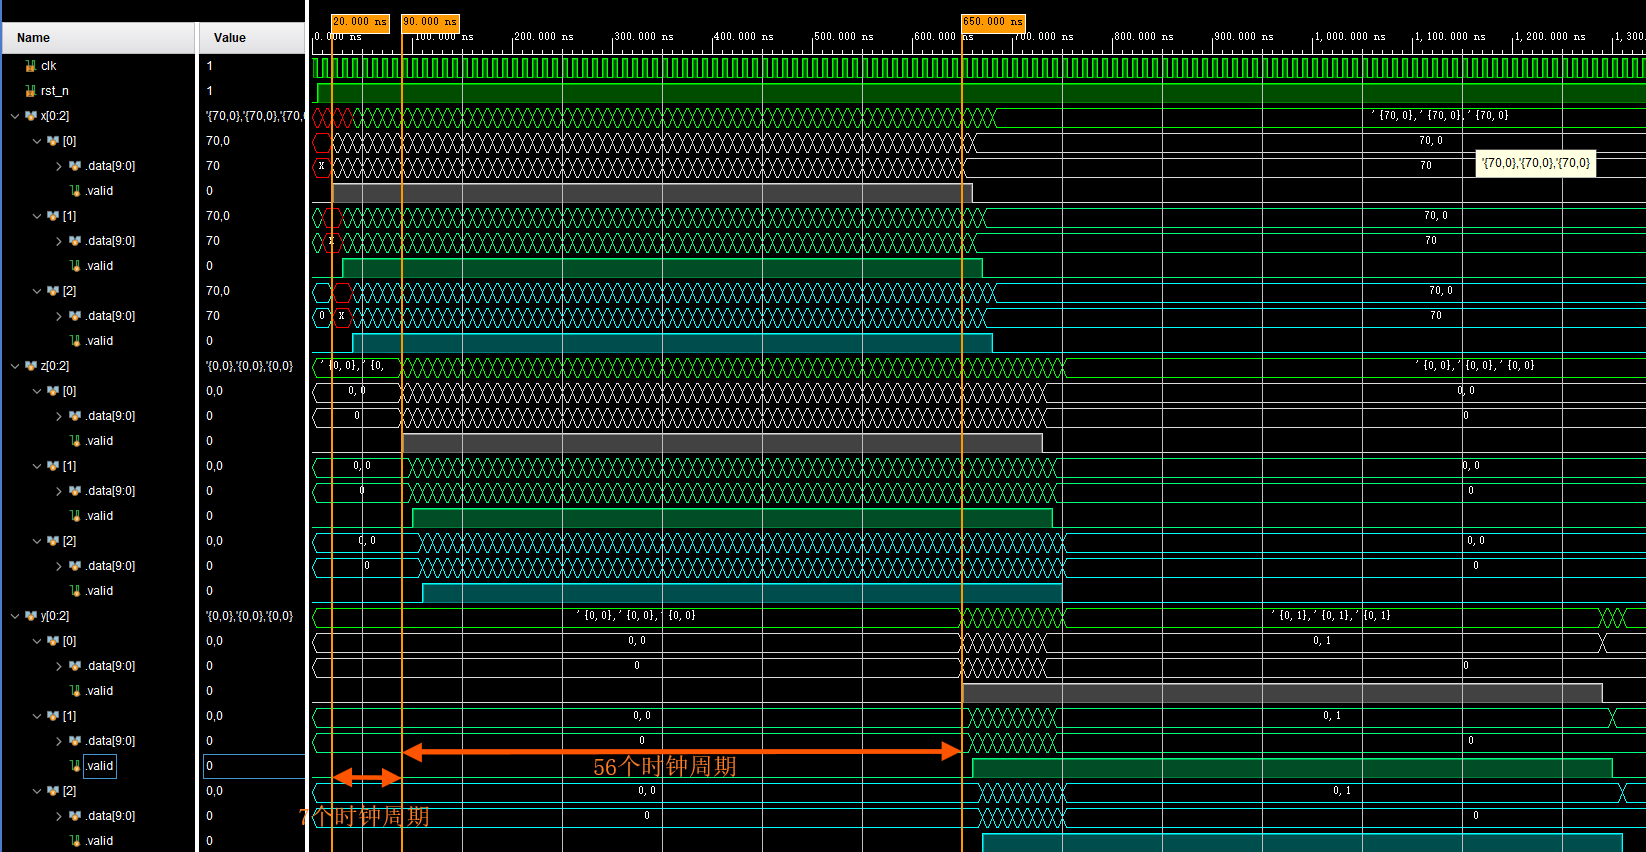
\includegraphics[scale=0.375]{./pictures/DCT模块仿真.png}
        \caption{DCT模块仿真波形}
        \label{DCTSimulationWave}
      \end{figure}

      \begin{figure}[H]
        \centering
        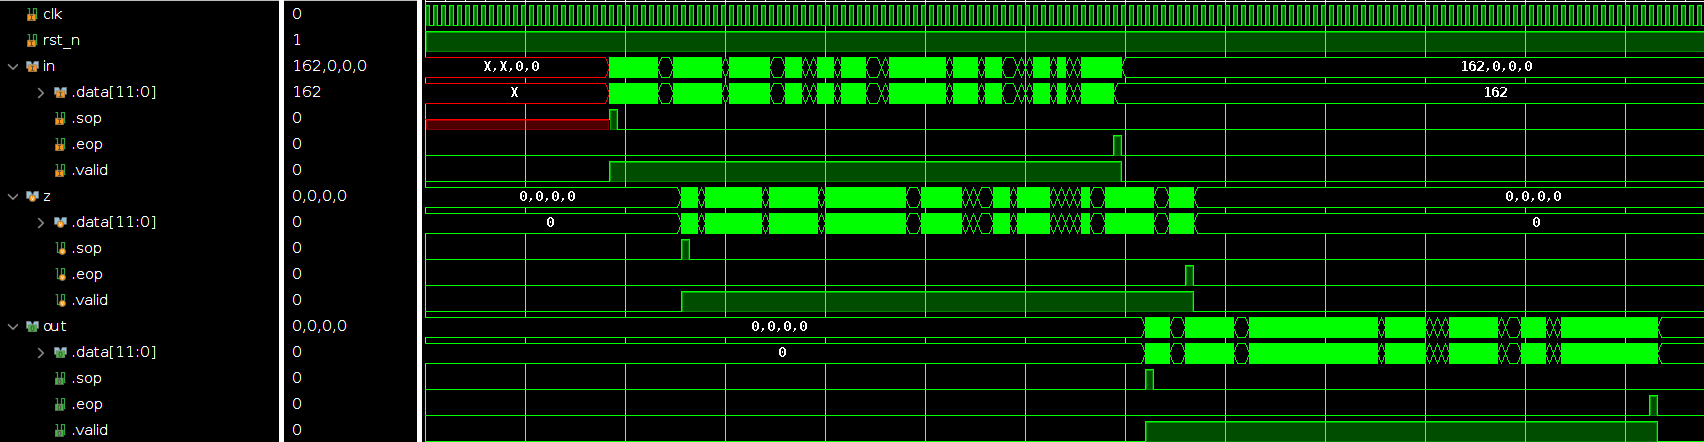
\includegraphics[scale=0.275]{./pictures/dct_wave.png}
        \caption{单个颜色通道仿真波形}
        \label{single color channal}
      \end{figure}

    下面验证计算结果的准确性,以如表(\ref{testMatrix})矩阵作为输入。
    与使用python的numpy库编写的DCT计算结果进行对比。
    \begin{table}[H]
      \caption{测试8×8单元测试输入}
      \label{testMatrix}
      \centering
      \begin{tabular}{cccccccc}
        \toprule
        \multicolumn{8}{c}{测试8×8单元测试输入}\\
        \midrule
        0 & 10 & 20 & 30 & 40 & 50 & 60 & 70 \\
        0 & 10 & 20 & 30 & 40 & 50 & 60 & 70 \\
        0 & 10 & 20 & 30 & 40 & 50 & 60 & 70 \\
        0 & 10 & 20 & 30 & 40 & 50 & 60 & 70 \\
        0 & 10 & 20 & 30 & 40 & 50 & 60 & 70 \\
        0 & 10 & 20 & 30 & 40 & 50 & 60 & 70 \\
        0 & 10 & 20 & 30 & 40 & 50 & 60 & 70 \\
        0 & 10 & 20 & 30 & 40 & 50 & 60 & 70 \\
        \bottomrule
      \end{tabular}
    \end{table}

    \begin{figure}[H]
      \centering
      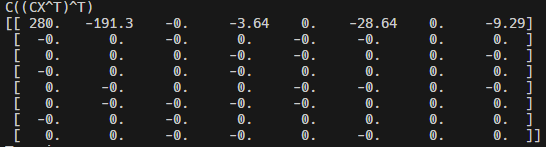
\includegraphics[scale=0.8]{./pictures/python脚本运行结果.png}
      \caption{python脚本运行结果}
      \label{py result}
    \end{figure}
    \begin{figure}[H]
      \centering
      \includegraphics[scale=0.3725]{./pictures/DCTSimulationResult.png}
      \caption{ DCT仿真结果波形}
      \label{result simulation}
    \end{figure}

    图\ref{py result}为python脚本运行结果,图\ref{result simulation}为DCT模块计算结果的波形,
    可以粗略地估计模块的运算结果和实际的运算结果存在$\stackrel{+}{-}5$的误差。这是由于对定
    点数运算结果进行截位导致的。本模块使用10位数据进行运算因此误差的
  \subsection{zigzag扫描及量化模块}
    \vspace{1em}
    zigzag扫描器的仿真波形如图\ref{scannerWave}所示。可以明显看出坐标值x和y是按照zigzag扫描
    的顺序进行变化的。
      \begin{figure}[H]
        \centering
        \includegraphics[scale=0.4]{./pictures/scannerWave.png}
        \caption{Zigzag 仿真波形图}
        \label{scannerWave}
      \end{figure}

    从DCT模块输出的数据经过zigzag和量化模块的后输出波形如图\ref{quantizer wave}所示,可以看
    出经过zigzag扫描和量化后出现连续的0值。
    \begin{figure}[H]
      \centering
      \includegraphics[scale=0.32]{./pictures/quantizer_wave.png}
      \caption{量化器输出波形}
      \label{quantizer wave}
    \end{figure}
  \subsection{熵编码模块仿真}
    \vspace{1em}
    \begin{figure}[H]
      \centering
      \includegraphics[scale=0.25]{./pictures/temp_wave.png}
      \caption{中间码生成模块仿真波形}
      \label{temp wave}
    \end{figure}
    如图\ref{temp wave}所示,中间码生成模块接收量化输出,并将其非零值
    进行VLI编码,记录非零值前的零值的个数。
    \begin{figure}[H]
      \centering
      \includegraphics[scale=0.25]{./pictures/EOBGen_wave.png}
      \caption{EOB生成模块仿真波形}
      \label{EOBGen wave}
    \end{figure}
    如图\ref{EOBGen wave}所示,EOB输出器接收中间码生成模块的输出。如果
    存在EOB,将EOB前面的ZRL进行销毁,并输出EOB。
    \begin{figure}[H]
      \centering
      \includegraphics[scale=0.25]{./pictures/Huffman_wave.png}
      \caption{Huffman编码仿真波形}
      \label{Huffman wave}
    \end{figure}
    如图\ref{Huffman wave}所示,Huffman编码器接收EOB生成模块的输出。并将
    run值和有效长度值进行huffman编码再与VLI编码拼接输出,同时输出对应编码的
    有效长度。
    \begin{figure}[H]
      \centering
      \includegraphics[scale=0.25]{./pictures/splice_wave.png}
      \caption{不定长数据拼接模块仿真波形}
      \label{splice wave}
    \end{figure}
    如图\ref{splice wave}所示,该模块接收Huffman编码模块的输入,并更具有效长
    度进行拼接,当done信号有效时,说明单个8×8单元输入完毕。对拼接值进行输出
    同时输出对应有效长度。
\newpage
\section{FPGA实现与上板验证}
  本设计使用Smart ZYNQ SP开发板进行FPGA实现。该开发板搭载一颗ZYNQ XC7Z020-CLG484。
  本设计使用了该SOC的PL部分作为FPGA实现。在vivado软件中进行实现,最终实现的资源占
  用如图\ref{implementation}所示。
  \begin{figure}[H]
    \centering
    \includegraphics[scale=0.5]{./pictures/资源占用.png}
    \caption{资源占用}
    \label{implementation}
  \end{figure}

  本设计的时序分析报告结果如图/ref{timing}所示。
  \begin{figure}[H]
    \centering
    \includegraphics[scale=0.4]{./pictures/时序报告.png}
    \caption{时序报告}
    \label{timing}
  \end{figure}
  根据时序报告可以得出,本设计的保持时间余量WNS为5.847ns。本设计的fpga实现使用
  50Mhz作为时钟输入。由公式(\ref{Fmax})得出最大工作时钟约为70.65Mhz。
  \begin{equation}
    F_{max}=\frac{1}{T-{WNS}}
    \label{Fmax}
  \end{equation}


  \subsection{上板验证}
    本设计使用Smart ZYNQ SP开发板进行FPGA实现。该开发板搭载一颗ZYNQ XC7Z020-CLG484
    同时使用FT2232HQ提供了一路USB-UART接口。本设计的验证平台如图\ref{FPGA}所示。
    \begin{figure}[H]
      \centering
      \includegraphics[scale=0.40]{./pictures/验证平台.png}
      \caption{验证平台}
      \label{FPGA}
    \end{figure}

    \begin{figure}[H]
      \centering
      \includegraphics[scale=0.20]{./pictures/实机验证.jpg}
      \caption{实机验证}
      \label{fpga test}
    \end{figure}
    本系统在PC通过uart接口发生和接收原始图像和压缩数据。并在PC端进行解码验证功能正确性。


\newpage
  \vspace{1em}


\bibliographystyle{plain}
\addcontentsline{toc}{section}{参考文献}
\bibliography{references}
\end{spacing}

\newpage
\section*{致\ \ \ 谢}
\addcontentsline{toc}{section}{致谢}

  行文至此,意味着我的本科生涯与毕业论文即将画上句点。回首这段求学旅程,虽有艰辛,但更多
  的是成长与感动。在此,我谨向所有给予我帮助和支持的人致以最诚挚的感谢。首先,衷心感谢我
  的指导老师孙永坚老师,从选题定题、框架搭建到细节修改,您始终以严谨的学术态度和耐心的
  指导为我指明方向,您渊博的学识、敏锐的学术洞察力以及精益求精的治学精神,将永远激励我在
  未来的道路上砥砺前行。感谢我的同窗好友以及室友们,是你们在学术探讨中的思维碰撞让我受益
  匪浅,在低谷时的鼓励让我重拾信心,与你们共度的青春岁月,是我大学生活中最珍贵的财富。深
  深感谢我的父母和家人,二十余载无私的付出与包容,为我撑起一片追逐梦想的天空,你们的爱与
  支持,是我勇往直前的永恒动力。最后,向参与论文评审和答辩的各位专家老师致以谢意,感谢你
  们提出的宝贵意见,文中不足之处,责任皆在于我,未来将继续完善。以梦为马,不负韶华,愿将
  此文献给所有关心我的人,愿我们山水有相逢,未来皆可期。\vspace{1em} \\
  \begin{flushright}
    黄智为\\
    \today{}
  \end{flushright}
  
  
\end{document}
